\documentclass[aspectratio=43]{beamer}
\mode<presentation>
\usetheme{Madrid}
\usecolortheme{seahorse}
% \usepackage[table]{xcolor}
\usepackage{multimedia}
\usepackage{media9}
\usepackage[utf8]{inputenc}
\usepackage{amsmath}
\usepackage{lmodern}
% \usepackage[usenames, dvipsnames]{color}
\hypersetup{
  colorlinks=True,
  urlcolor=blue,
}

\usepackage{arydshln}
\usepackage{url}
\usepackage[absolute,overlay]{textpos}
% \usepackage[texcoord,grid,gridunit=mm,gridcolor=red!10,subgridcolor=green!10]{eso-pic}
\setlength{\TPHorizModule}{\textwidth}
\setlength{\TPVertModule}{\textwidth}

\graphicspath{{plots/}}

\setbeamercolor{CBwonb}{fg=white,bg=white!10!blue}
\setbeamercolor{CBronb}{fg=red,bg=white!10!blue}

\usepackage{tikz}
\usetikzlibrary{shapes,arrows,positioning}
\tikzstyle{startstop} = [rectangle, rounded corners, minimum width=1cm, minimum height=0.1cm,text centered, text width=2.5cm, draw=black, fill=red!30]
\tikzstyle{io} = [trapezium, trapezium left angle=70, trapezium right angle=110, minimum width=1cm, minimum height=0.1cm, text centered, text width=2.5cm, draw=black, fill=blue!30]
\tikzstyle{process} = [rectangle, minimum width=1cm, minimum height=0.1cm, text centered,text width=2.5cm, draw=black, fill=orange!30]
\tikzstyle{decision} = [circle, minimum width=1cm, minimum height=0.1cm, text centered,text width=2.5cm, draw=black, fill=green!30]
\tikzstyle{arrow} = [thick,->,text centered, color=blue, text width=2cm,>=stealth]

\newcommand{\Msun}{~{\rm M_\sun}}
\newcommand{\hMsun}{~h^{-1}\>{\rm M_\odot}}
\newcommand{\Mpc}{~h^{-1}~{\rm Mpc}}
\newcommand{\Kpc}{~h^{-1}~{\rm kpc}}


\title[]{The Three Hundred}
\subtitle{A large galaxy cluster catalogue for cosmological and astrophysical applications.}
\author[Email: weiguang.cui@uam.es]{{\Large \bf Weiguang Cui},\inst{*} \footnote{\url{https://weiguangcui.github.io}} \\
  In collaboration with the core team (Alexander Knebe, Frazer Pearce and  etc.) of the 300 project}
\institute[]{
  \inst{*}
  Departamento de F\'isica Te\'{o}rica, \\
  Universidad Aut\'{o}noma de Madrid, 28049 Madrid, Spain
}
\date[]{Purple mountain Observatory, Nanjing, 19, Oct. 2018 \\
Main results come from \hyperref{http://adsabs.harvard.edu/abs/2018MNRAS.480.2898C}{}{}{Cui et al. 2018, MNRAS, 480, 2898}, \hyperref{http://adsabs.harvard.edu/abs/2018arXiv180905244W}{}{}{Wang et al. 2018}, Mostoghiu et al. 2018, Arthur et al. to be submitted and Li et al. in prep.}
\logo{
\includegraphics[height=1cm]{logo_uam.jpg}}

%%%%%%%%%%%%%%%%%%%%%%%%%%%%%%%%%%%%%%%%%%%%%%%%%%%%%%%%%%%%%%%%%%%%%%%%%
\begin{document}
  \frame{\titlepage}

%----------------------------------
\section{Introduction} \label{sec:1}
\begin{frame}
  \begin{figure}
    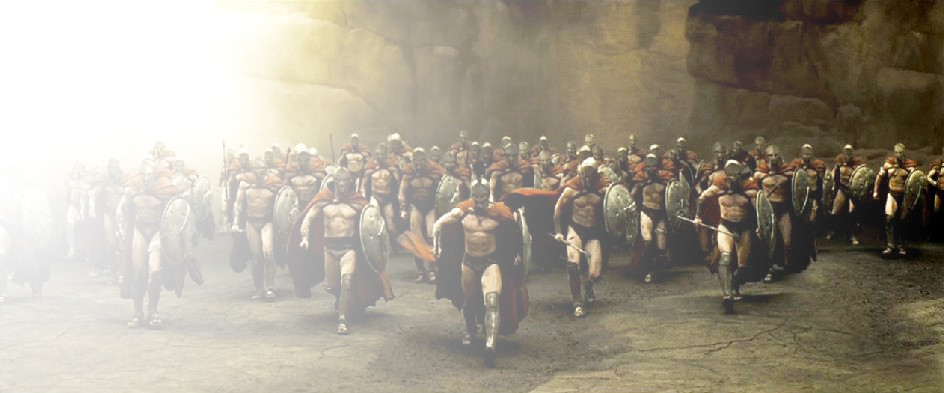
\includegraphics[width=\textwidth]{The300}
    \begin{textblock*}{0.5cm}(6.15cm,3.5cm) %(7.7cm,3.8cm) % {block width} (coords)
      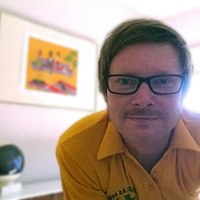
\includegraphics[width=0.5cm]{A_Knebe.jpg}
    \end{textblock*}
    \begin{textblock*}{0.5cm}(2.0cm,3.2cm) %(2.7cm,3.5cm) % {block width} (coords)
      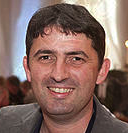
\includegraphics[width=0.5cm]{chris2.png}
    \end{textblock*}
    \begin{textblock*}{0.5cm}(4.4cm,3.3cm) %(5.7cm,3.6cm) % {block width} (coords)
      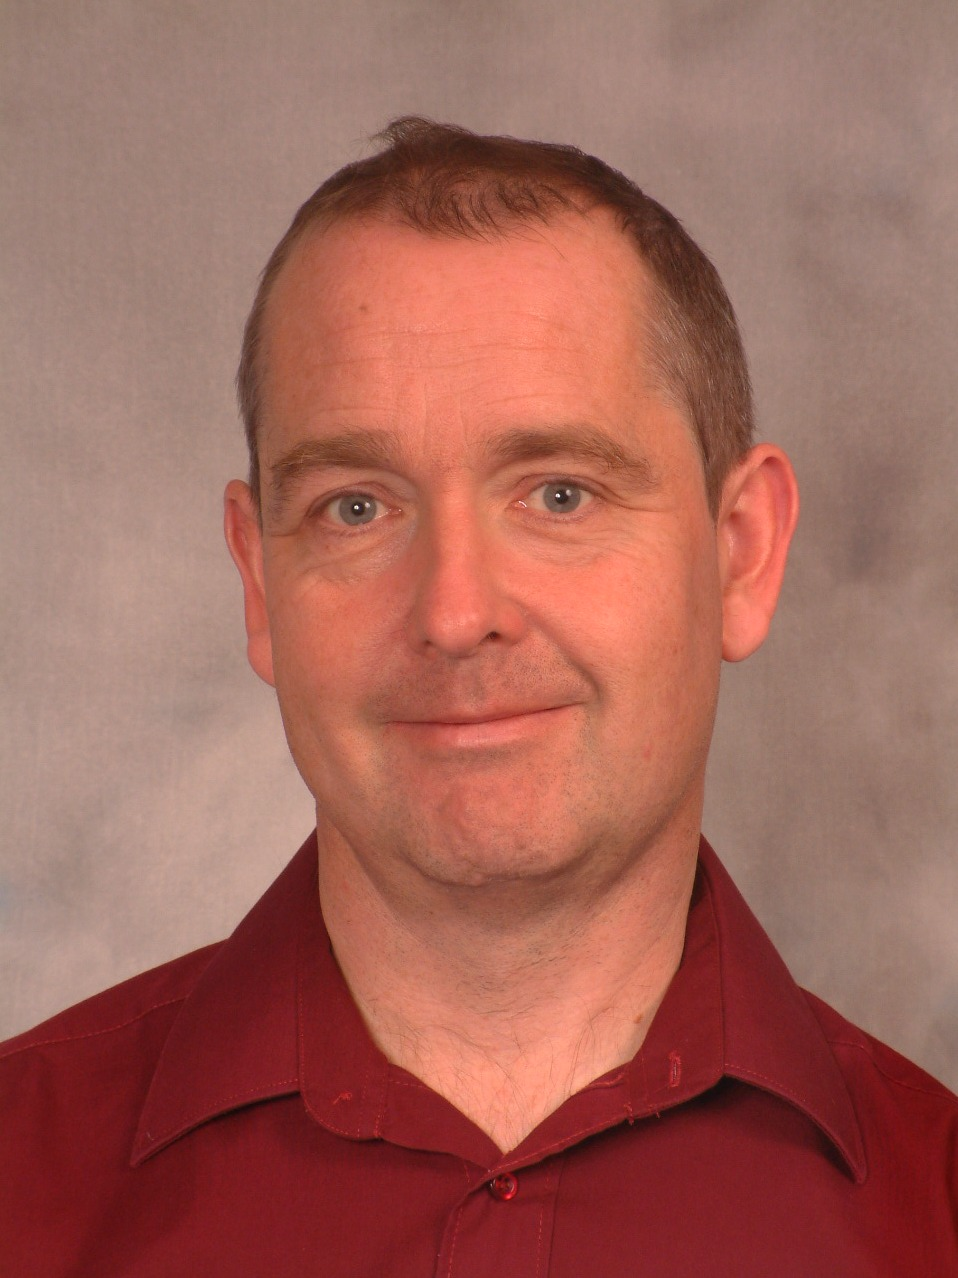
\includegraphics[width=0.5cm]{frazer.jpg}
    \end{textblock*}
    \begin{textblock*}{0.5cm}(7.7cm,3.3cm) %(9.7cm,3.4cm) % {block width} (coords)
      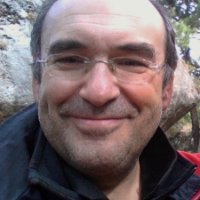
\includegraphics[width=0.5cm]{gustavo.jpg}
    \end{textblock*}
    \begin{textblock*}{0.5cm}(9.5cm,3.2cm) %(11.9cm,3.5cm) % {block width} (coords)
      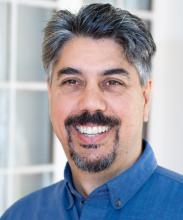
\includegraphics[width=0.5cm]{Dave}
    \end{textblock*}
    \caption{Join Us!}
  \end{figure}
\end{frame}
\begin{frame}
  \frametitle{Background: Cluster of Galaxies:}
    \begin{itemize}
      \item<1-> Galaxy cluster is the final state of the hierarchical structure formation.
      \item<2-> Typically a few Mpc across, contain $\sim$ 100 - 1000 luminous galaxies and many more dwarfs, masses $\gtrsim 10^{14.5} M_{\odot}$.
      \item<3-> Dark matter: $\sim 85 \%$, gas: $\sim 13 \%$, star: $\sim 1 - 2 \%$.
      \item<4-> It provides plentiful information for baryonic processes, galaxy formation and cosmology models.
      \item<5->[]
        \begin{figure}
          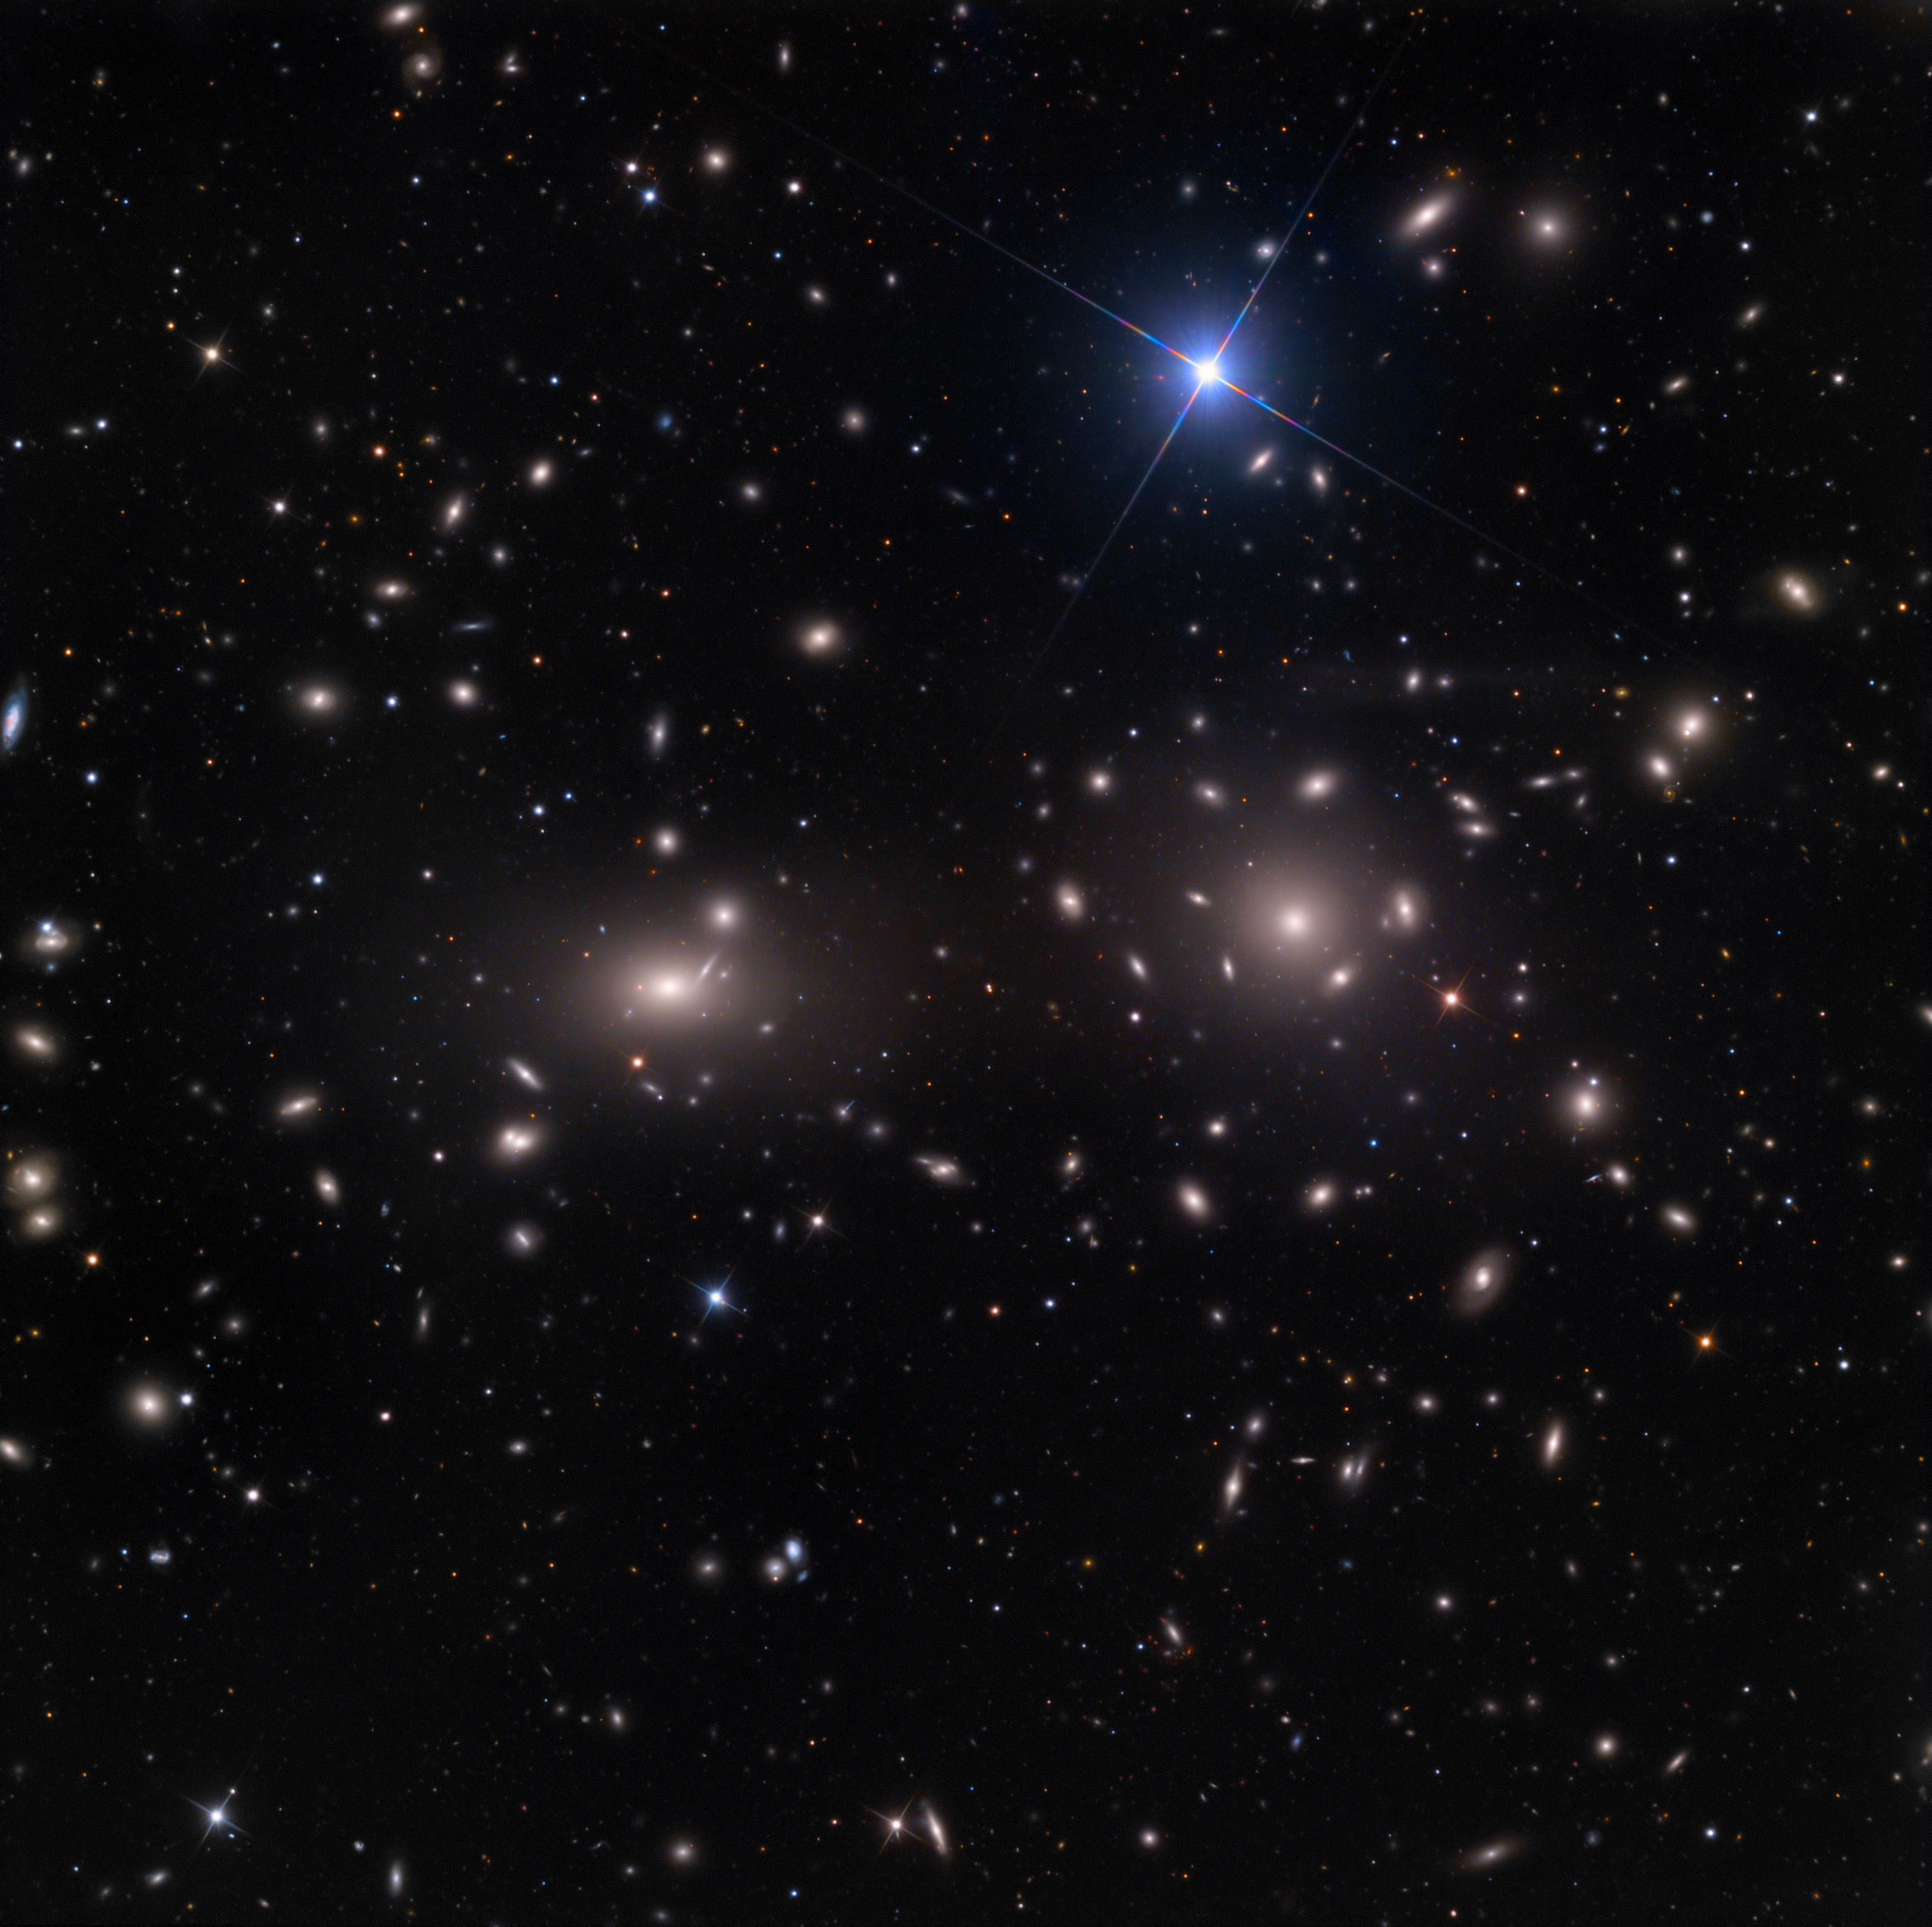
\includegraphics[width=0.292\textwidth]{Coma-SDSS.jpg}
          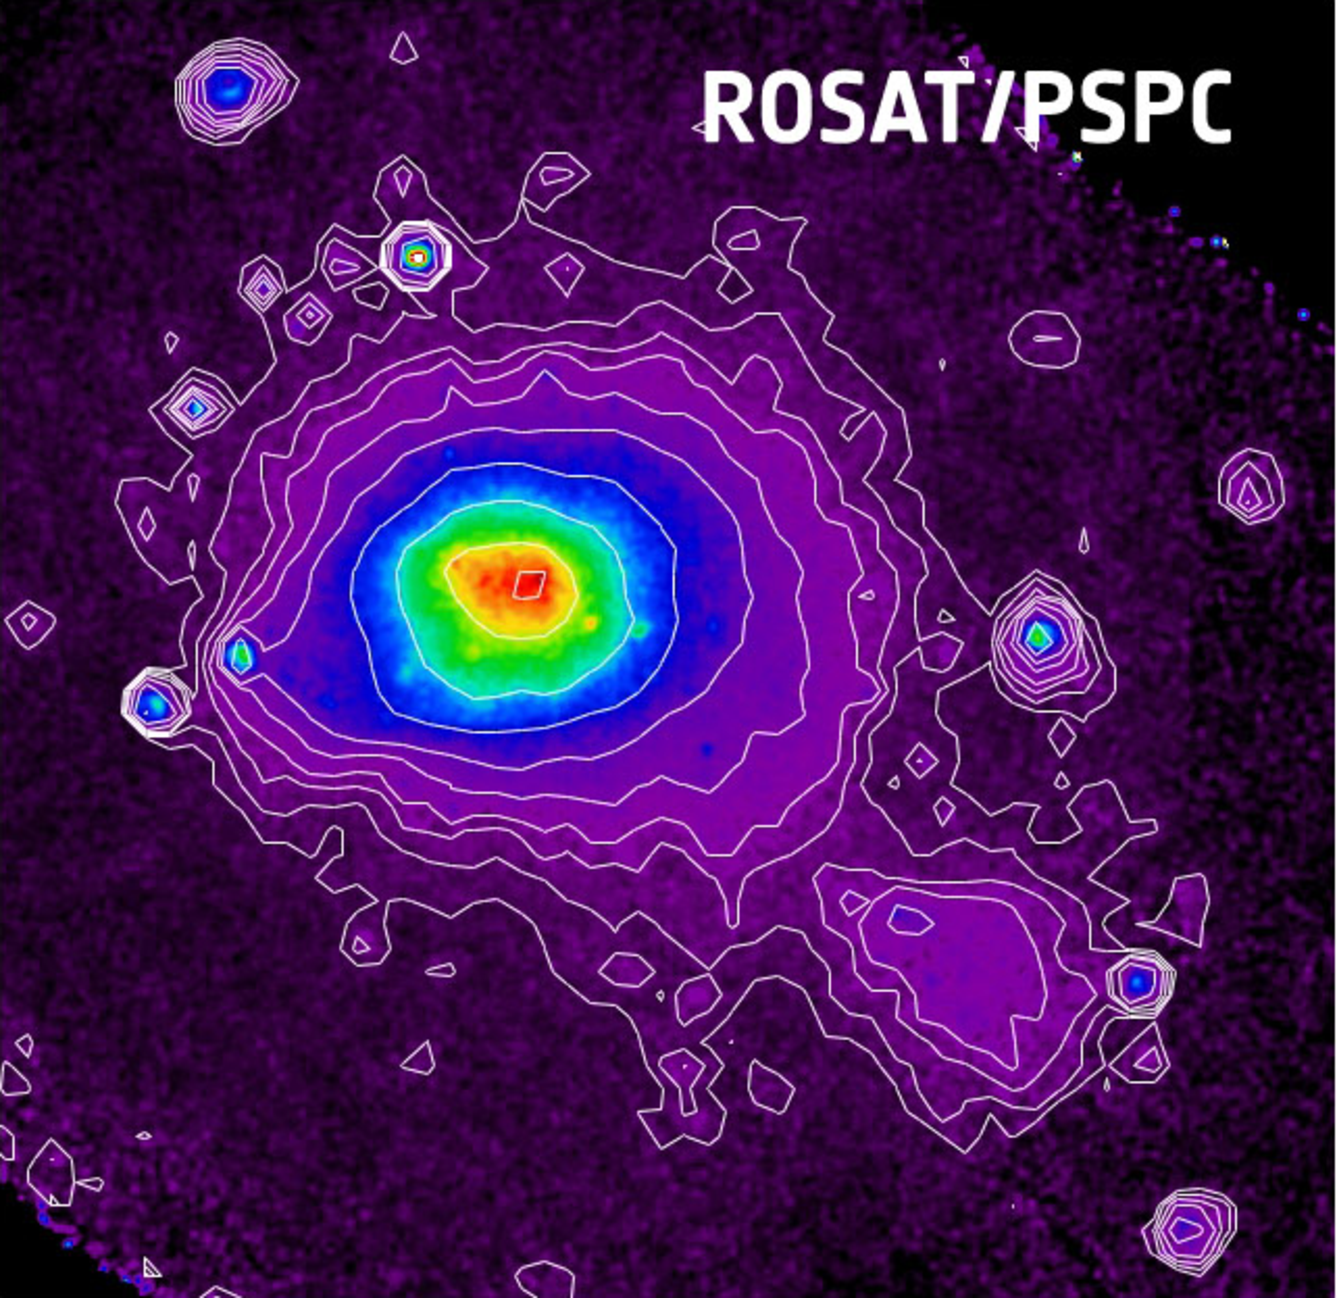
\includegraphics[width=0.3\textwidth]{Coma-Rosat.pdf}
          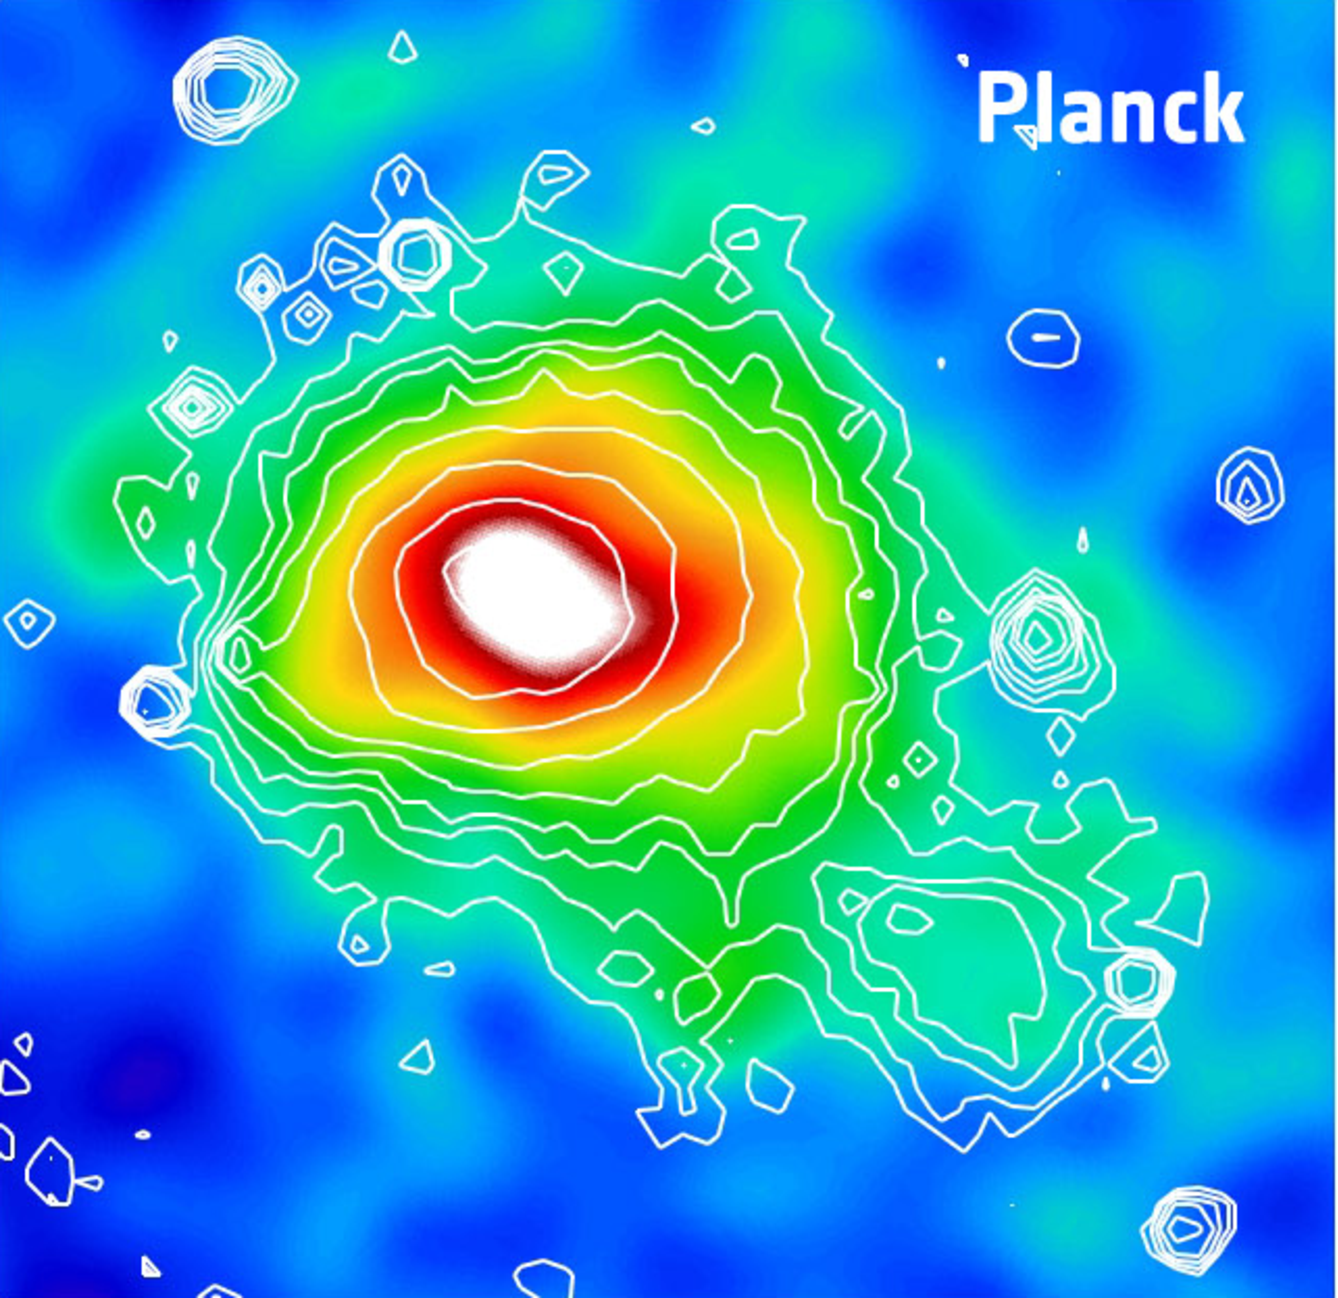
\includegraphics[width=0.3\textwidth]{Coma-Planck.pdf}
          \vspace{-0.4cm}
          \caption{The Coma cluster.}
        \end{figure}
    \end{itemize}
\end{frame}

\begin{frame}
  \frametitle{Background: Cluster of Galaxies:}
  % \only<1>{
  % \begin{block}{The importance of galaxy clusters}
  %   \begin{itemize}
  %     \item Constrain cosmology models.
  %     \item Study galaxy formation and improve the galaxy formation models.
  %     \item investigate and understand the small scale baryonic physics.
  %   \end{itemize}
  % \end{block}
  % }
  \only<1>{
  {\bf To understand these observational results, especially how they are formed, we need simulations.}

  \begin{center}
    \movie[loop,autostart]{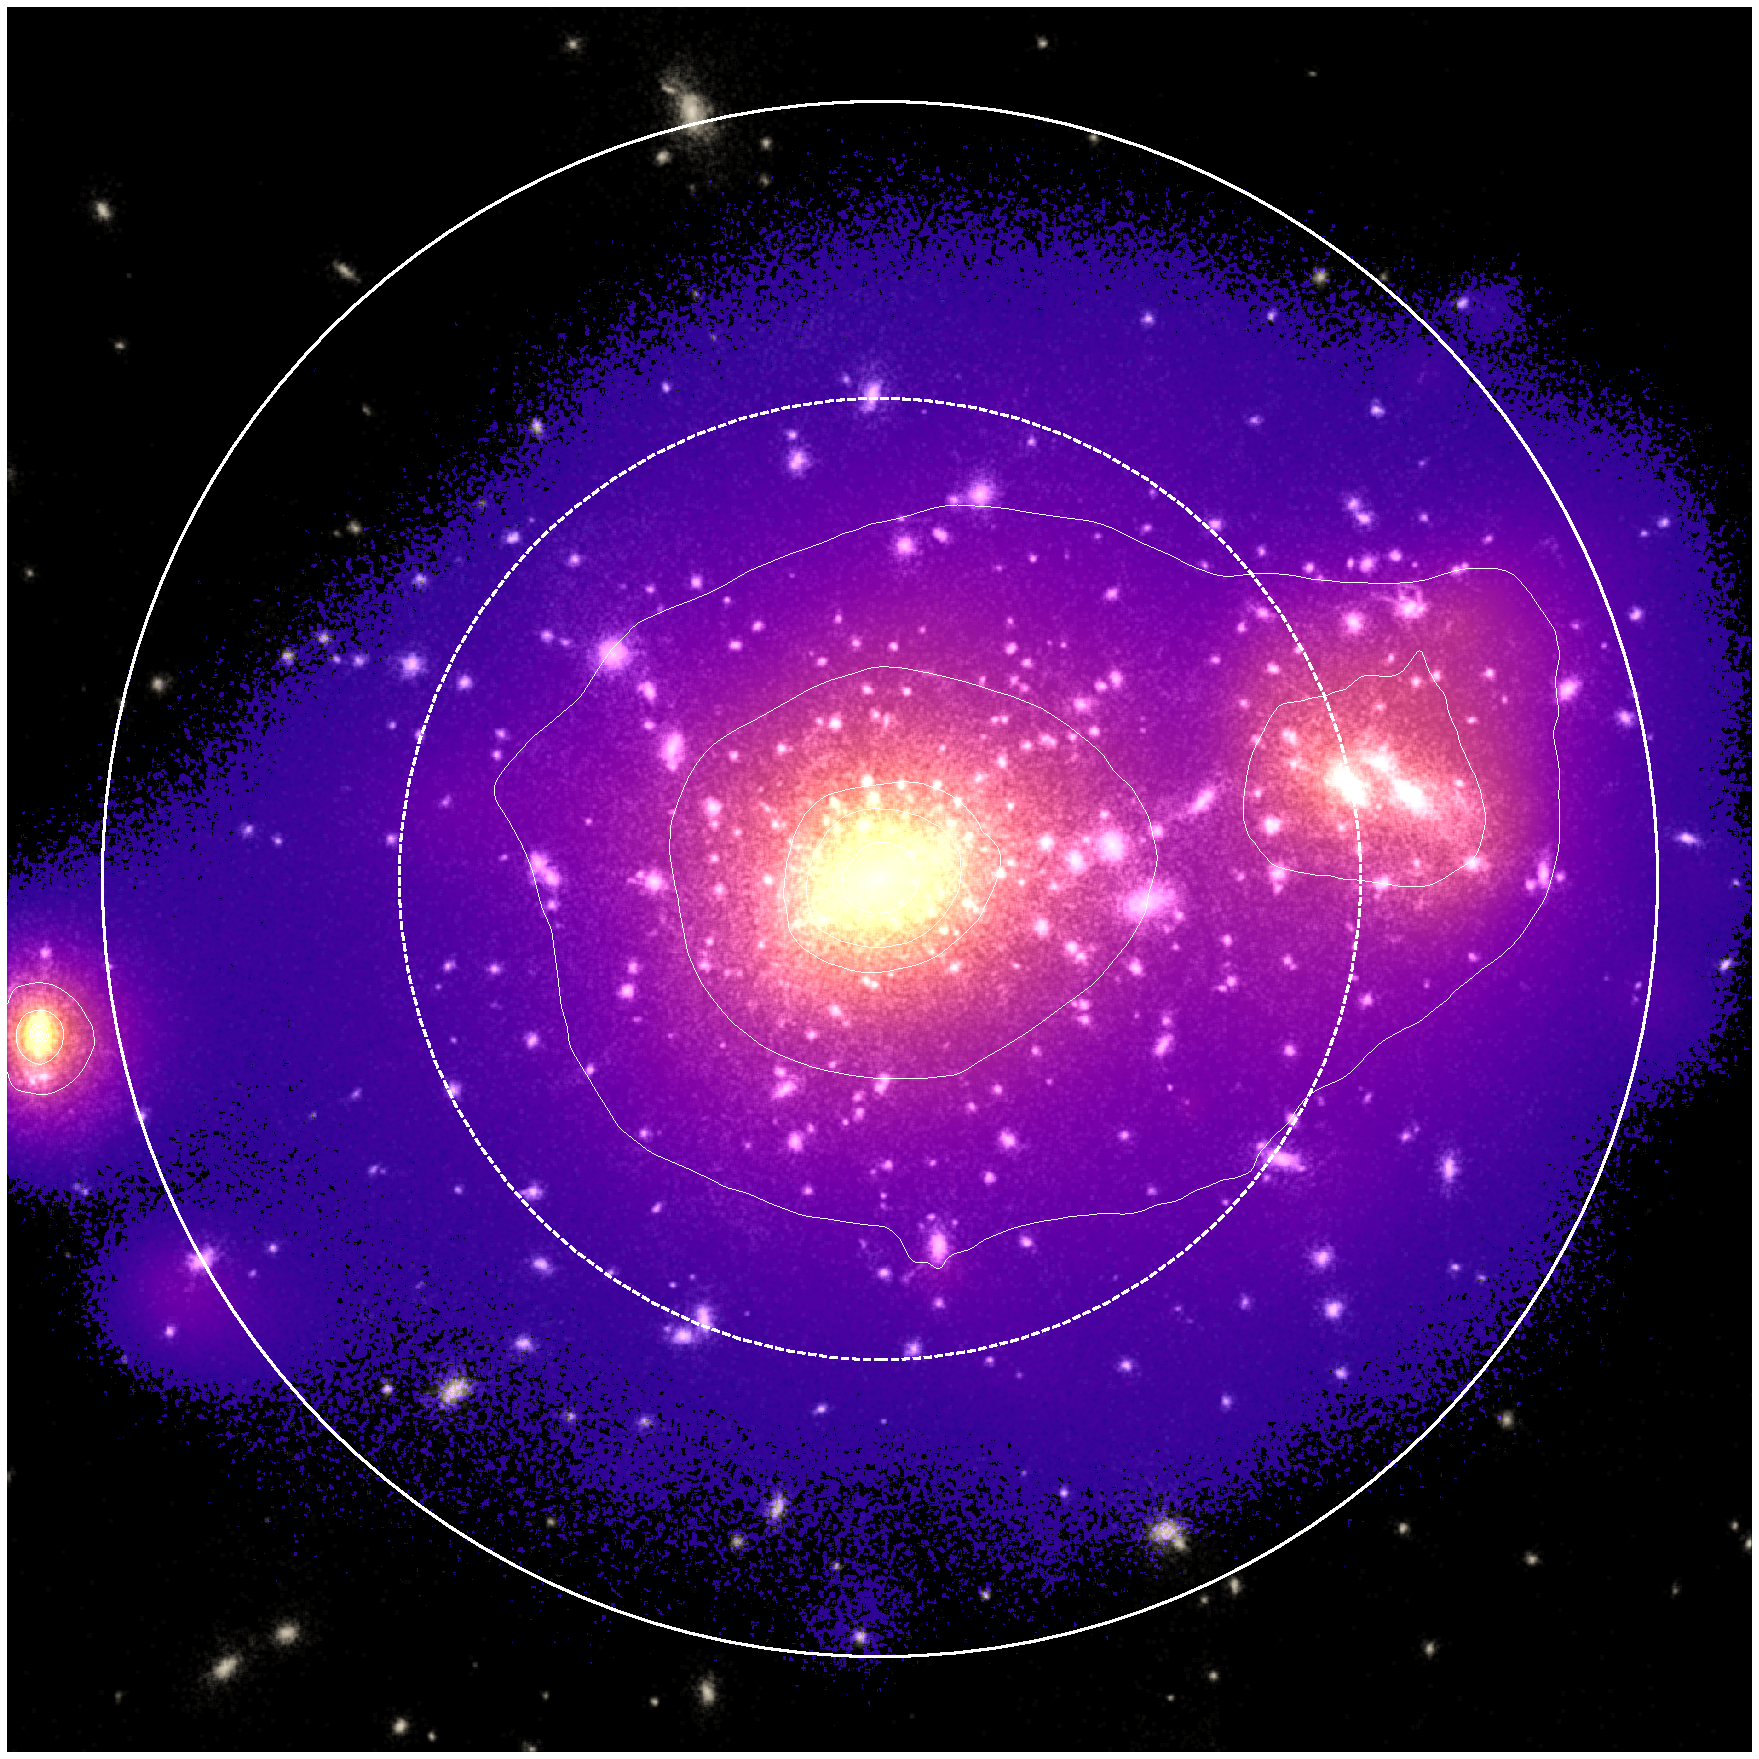
\includegraphics[width=0.6\textwidth]{G3X-17-image.pdf}}{plots/NewMDCLUSTER_0017.mp4}
  \end{center}

  % This require Adobe PDF viewer, evince not working!
  % \begin{center}
  % \includemedia[
  % 	width=0.6\linewidth, %height=0.3\linewidth,
  % 	activate=pageopen,
  % 	addresource=plots/NewMDCLUSTER_0017.mp4,
  %   flashvars={
  %     source=plots/NewMDCLUSTER_0017.mp4
  %    &autoPlay=true % start playing on activation
  %    &loop=true
  %   }
  % ]{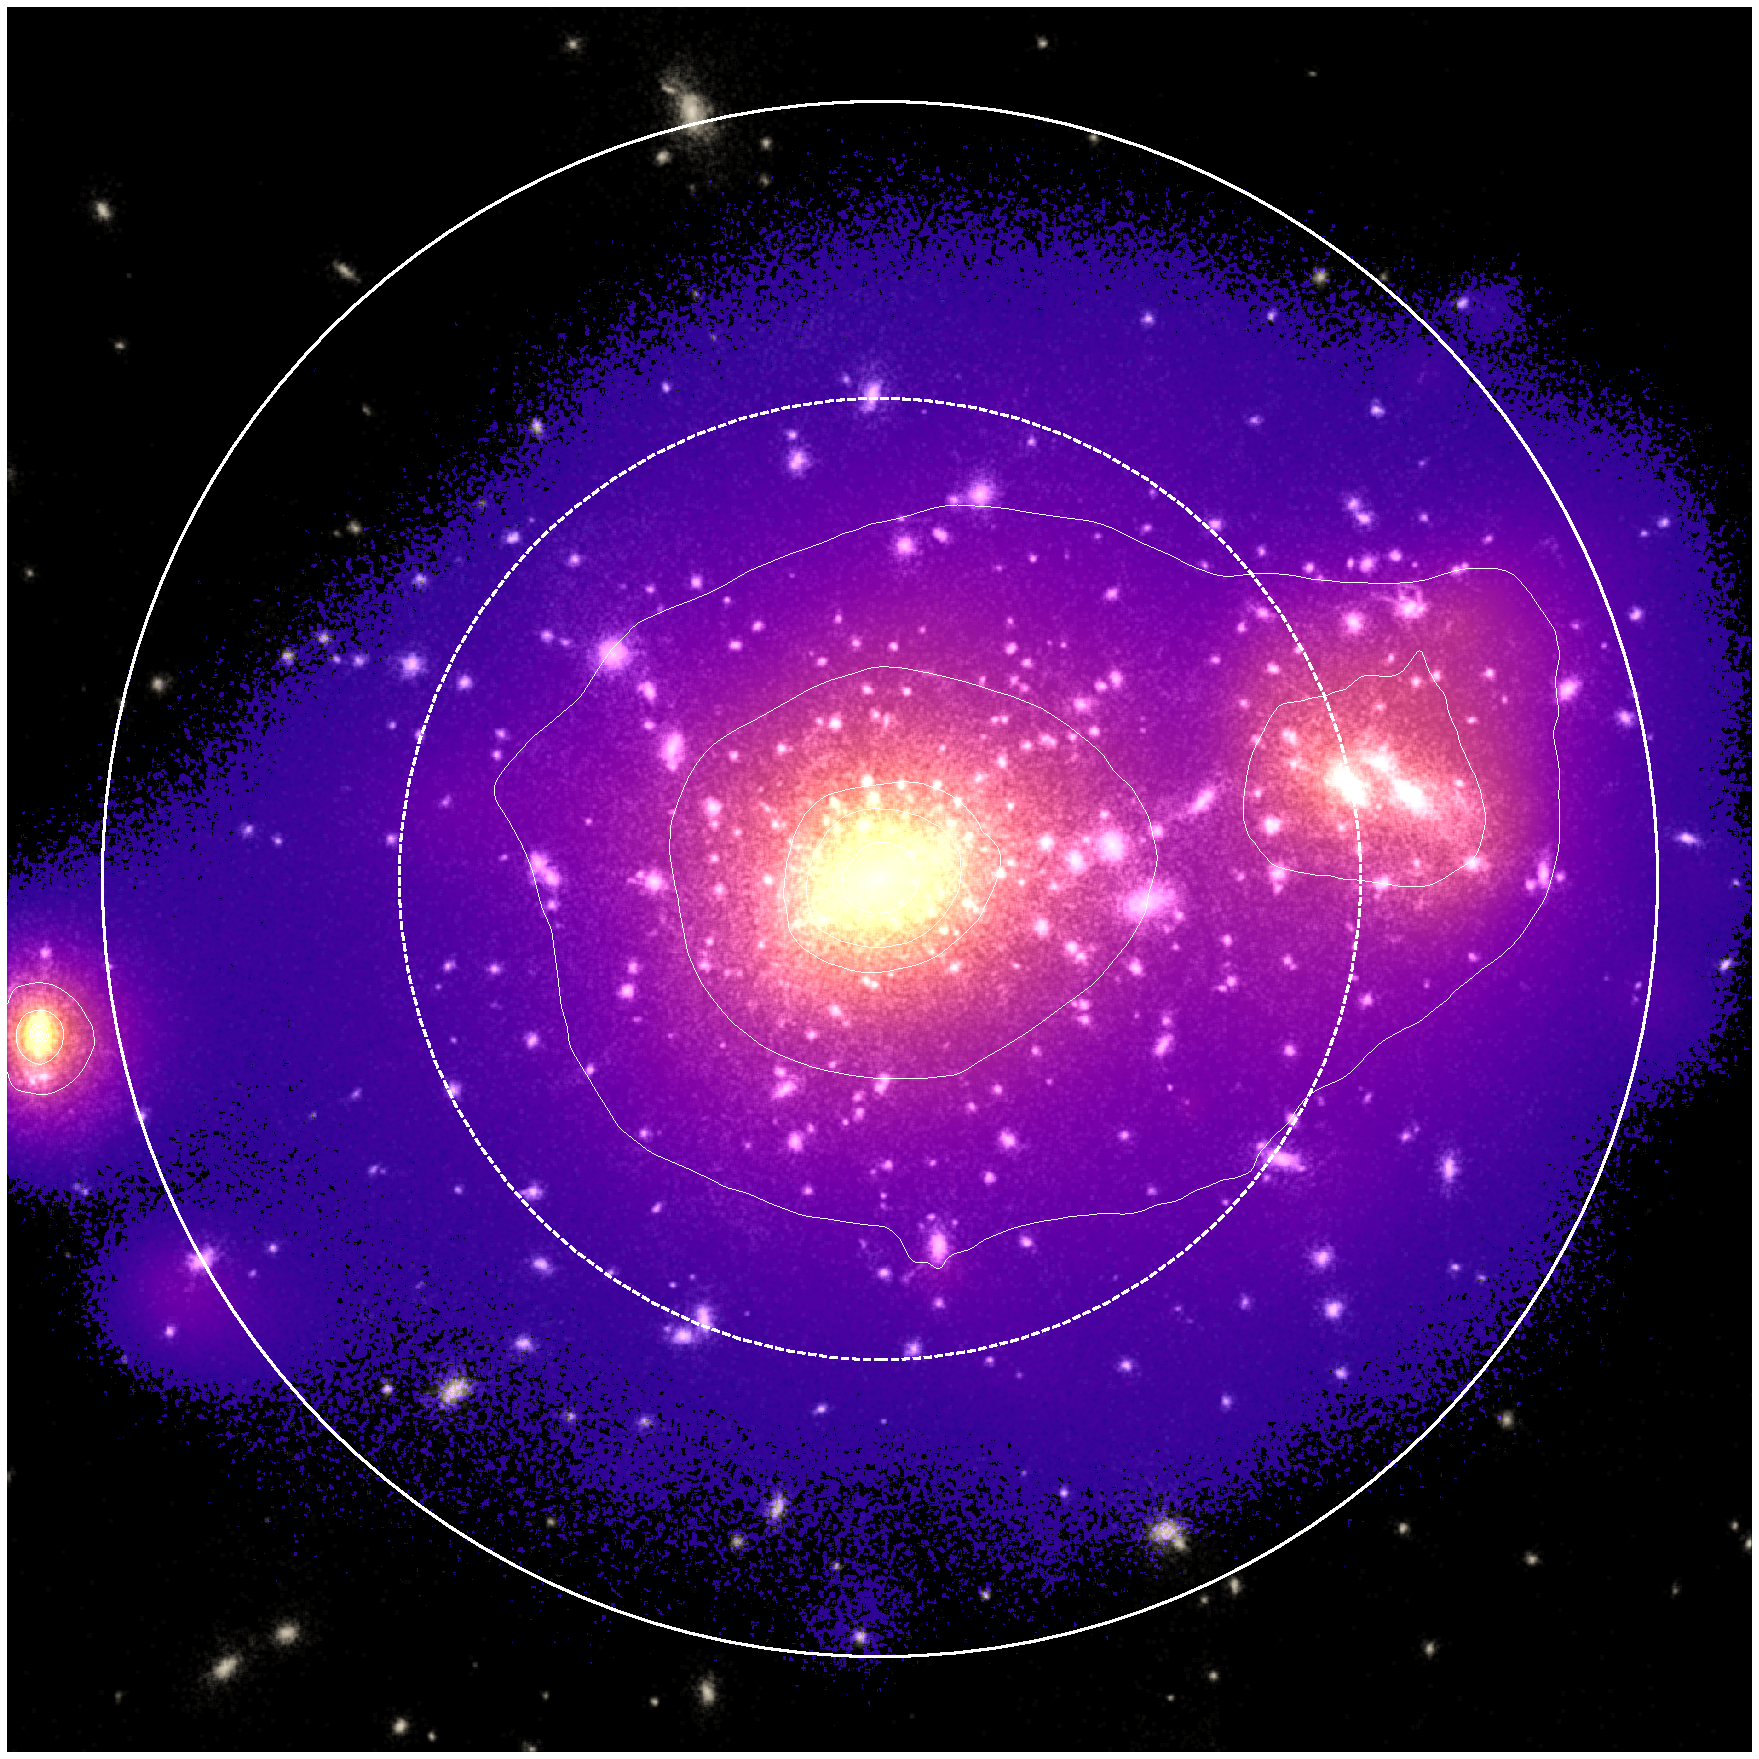
\includegraphics[height=0.3\linewidth]{G3X-17-image.pdf}}{VPlayer.swf}
  % \end{center}

  \begin{textblock}{0.2}(0.05,0.4)
    {\scriptsize Simulated Cluster 17 from the 300 project \\ credit: Gustavo Yepes.}
  \end{textblock}
  }
\end{frame}

\begin{frame}
  \frametitle{The motivation of the Three Hundred: A successor of the {\sc nIFTy} project}
  \only<1>{
    \begin{center}
      {\Large \bf The {\sc nIFTy} galaxy cluster comparison project}\footnote{\scriptsize Ref: Sembolini et al. 2016a,b; Elahi et al. 2016; Cui et al. 2016; Arthur et al. 2017}
    \end{center}
    \alert{11} different (in both algorithms and baryon models) simulation codes are used to simulate the same galaxy cluster.
    \begin{figure}
      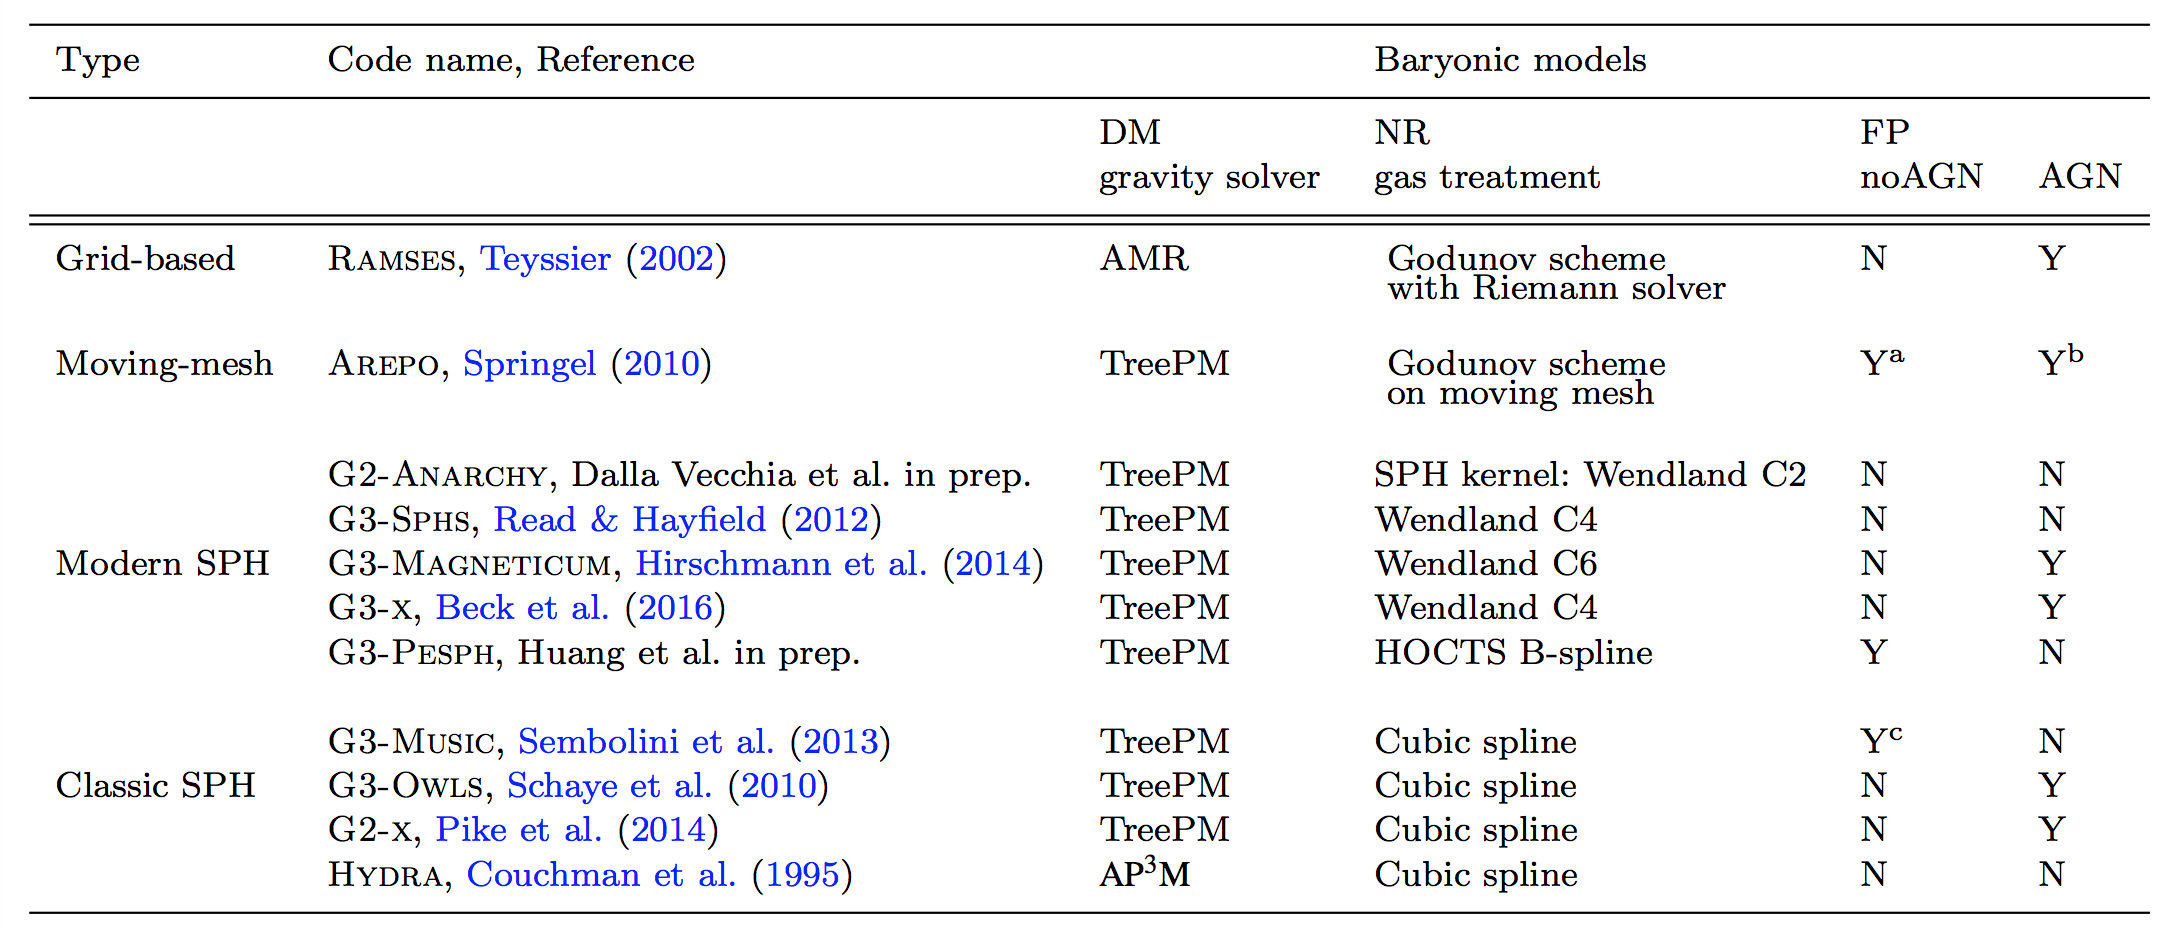
\includegraphics[width=0.9\textwidth]{nifty-codes.png}
      % \caption{{\small Sembolini et al. 2016a, 2016b.}}
    \end{figure}
  }
  \only<2>{
    \begin{center}
      {\Large \bf What did we find? I}
    \end{center}
    {\scriptsize
    \begin{itemize}
      \item The modern SPH codes produce correct entropy profiles as AMR, moving mesh.
      \item The baryon models have larger effects than the fluid simulating techniques by mixing the entropy profiles.
    \end{itemize}}
    \begin{figure}
      \vspace{-0.2cm}
      \includegraphics<2>[width=0.36\textwidth]{nifty-entropy.png}
      \includegraphics<2>[width=0.45\textwidth]{nifty-entropy-fp.png}\vspace{-0.4cm}
      % \caption{{\scriptsize Entropy profile. Ref: Sembolini et al. 2016a,b}}
    \end{figure}
    \begin{textblock}{0.12}(0.01,0.4)
      {\scriptsize  Entropy profile. \\ Ref: Sembolini et al. 2016a,b.}
    \end{textblock}
  }
  \only<3>{
    \begin{center}
      {\Large \bf What did we find? II}
    \end{center}
    % {\scriptsize
    % \begin{itemize}
    %   \item Different baryon models produce similar global properties, large scatter at small scales.
    % \end{itemize}}
    \begin{figure}
      \includegraphics<3>[width=0.45\textwidth]{be-dp}
      % \includegraphics<2>[width=0.45\textwidth]{nifty-entropy-fp.png}
    \end{figure}
    \begin{textblock}{0.25}(0.05,0.4)
      {\scriptsize E.g. Baryon effects on density profile. \\ Ref: Cui et al. 2016}
    \end{textblock}
    }
  \only<4->{
    \begin{center}
      {\Large \bf What's next?}
    \end{center}
    \alert{Aim: } to understand the formation and evolution of galaxy clusters.
    \begin{itemize}
      \item Comparisons between models to understand the theoretical predictions.
      \item Comparisons between models and observations to constrain the models.
    \end{itemize}

  ~}
  \only<5>{
  \begin{center}
      \alert{\Large A large cluster sample!}
  \end{center} }
  % \begin{enumerate}
  %   \item \alert{Code} My own SSP code -- pymgal (inherited from EzGal)
  %   \item \alert{Location} \path{~/TheThreeHundred/maps/CCD/<simulation code name>/NewMDCLUSTER_XXXX/}
  %   \item \alert{Notes}
  %   \begin{itemize}
  %     \item 1) 5 SDSS + 3 HST filters are provided. Mass + age + metal in
  %   \end{itemize}
  % \end{enumerate}
\end{frame}

\begin{frame}
  \frametitle{Other works}
  \begin{table}
    \fontsize{7}{7}\selectfont
    \caption{Cluster projects}
    \begin{tabular}{llll}
      \hline
      Name & N & mass range & resolution ($M_{DM}$)\\
      \hline
      MUSIC\footnote{No AGN}, Sembolini et al. 2013 & 500 & $10^{14} < M_v < 2\times10^{15} \hMsun$ & $1.03\times 10^9 \hMsun$ \\
      Dianoga, Planelles et al 2013 & 29 & $M_{500} > 2\times10^{14} \hMsun$ & $8.5\times 10^8 \hMsun$\\
      Rhapsody-G, Hahn et al. 2017 & 10 & $M_v \sim 10^{15} \hMsun$ & $8.3\times 10^8 \hMsun$\\
      MACSIS,  Barnes et al. 2017a & 390 & $M_{FoF} > 10^{15} \hMsun$ & $4.4\times 10^9 \hMsun$\\
      C-EAGLE, Barnes et al. 2017b & 30 & $10^{14} < M_{200} < 2.5\times10^{15} \hMsun$ & $10^7 \hMsun$\\
      Hydrangea\footnote{Slightly different to EAGLE in AGN feedback}, Bahe et al. 2017 & 24 & $10^{14} < M_{200} < 2\times10^{15} \hMsun$ & $10^7 \hMsun$\\
      % The 300\footnote{Multiple hydro-simulation codes + SAMs}, Cui et al. 2018 & 324 & $M_{200} > 6.4\times10^{14} \hMsun$ & $1.3\times 10^9 \hMsun$\\
      \hline
    \end{tabular}
  \end{table}
\end{frame}

\section{The Three Hundred}
\begin{frame}
  \frametitle{The advantage of the Three Hundred: Basic information}
  \begin{itemize}
    \item<1-> {The most massive ($M_{vir} > 8\times 10^{14} \hMsun$) \alert{324} clusters are selected from the MultiDark simulation(MDPL2)\footnote{\url{https://www.cosmosim.org}}.}
    \item<1-> {The zoomed-in ICs are generated by cutting a spherical region with a radius of \alert{$15 \Mpc$} from the cluster center.}
    \item<2|only@2>[]{
      \begin{center}
        \begin{tikzpicture}
            \node[anchor=south west,inner sep=0] at (0,0) {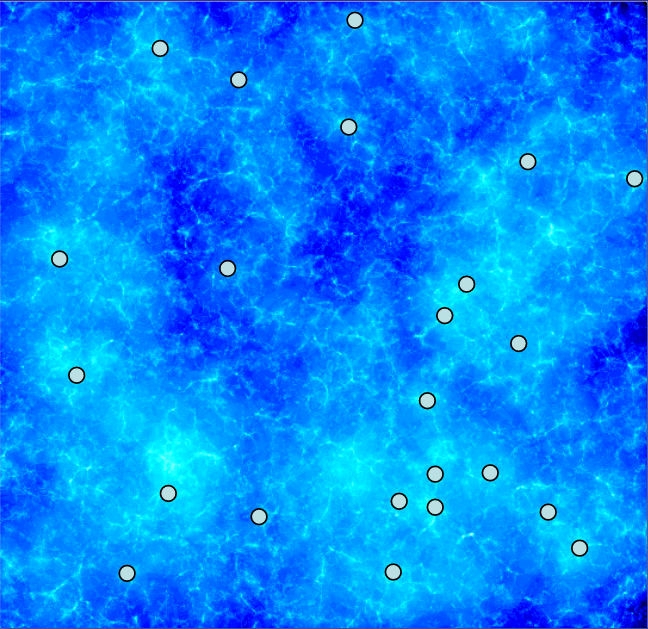
\includegraphics[width=0.6\linewidth]{MDPL2}};
            \draw[magenta,thick] (1.76,1.45) circle (0.2cm);
        \end{tikzpicture}
    \end{center}}
    \item<3|only@3>[]{
      \begin{table}
        \fontsize{10}{10}\selectfont
        \caption{Parameters of the Three Hundred simulations}
        \begin{tabular}{lll}
          \hline
          Parameter& Value & Description\\
          \hline
          $\Omega_M$ & 0.307 & Total Matter density parameter\\
          $\Omega_B$ & 0.048 & Baryon density parameter\\
          $\Omega_\Lambda$ & 0.693 & Cosmological Constant density parameter\\
          $h$ & 0.678  & Hubble constant in units of 100 km/s/Mpc\\
          $\sigma_8$ & 0.823 & Normalization of Power spectrum\\
          $n_s$ & 0.96  & Power index\\
          % $f_B$ & 0.0696&  Cosmic Baryon Fraction\\
          $z_{init}$ & 120 & Initial redshift of the simulations \\
          $\epsilon_{phys}$ & 6.5 & Plummer equivalent softening in $\Kpc$ \\
          % Box size & 1 $h^{-1} Gpc$ (15 $\Mpc$) & The MDPL2 simulation box on one side (the radius for each re-simulation region) \\
          Particle mass & $2.36 \ (12.7) $ & gas (dark matter) particle mass in [$10^8 \hMsun$]\\
          \hline
        \end{tabular}
      \end{table}}
\end{itemize}
% \vspace{-0.6cm}
\end{frame}

\begin{frame}
  \frametitle{The advantage of the Three Hundred: theoretical models}
  \vspace{-0.8cm}
  \begin{columns}[t]
    \begin{column}{0.5\textwidth}
      \begin{block}{hydrodynamical simulations with baryonic models:}
        {\sc Gadget-\alert{MUSIC}}: classic SPH method. Radiative cooling, star formation with both thermal and kinetic Supernove (SN) feedback.

        {\sc Gadget-\alert{X}}: modern SPH with the Wendland C4 kernel. Gas cooling with metal contributions, star formation with chemical enrichment, SN feedback with AGB phase, and AGN feedback.

        {\sc GIZMO:} running.

        {\sc Gadget-PESPH:} running.
      \end{block}
    \end{column}
    \begin{column}{0.48\textwidth}
      \begin{block}{SAMs from MultiDark-Galaxies:}
        Three different models \alert{\sc Galacticus}, \alert{\sc SAG} and \alert{\sc SAGE} (see Knebe et al. 2018 for details) are applied on the cosmological MultiDark simulation.

        {\sc Galacticus:} (Benson 2012) no calibration. only orphan galaxy.

        {\sc SAG:} (Cora et al. 2018) calibrated to observation. orphan galaxy + ICL.

        {\sc SAGE:} (Croton et al. 2016) no calibration. no orphan galaxy, only ICL.

        Notes: We select these catalogues from the same regions as the hydrodynamical simulations.
      \end{block}
    \end{column}
  \end{columns}
  % Let me know if you are interesting to run your model for the MultiDark simulation / 300 clusters.
\end{frame}
\begin{frame}
  \frametitle{The advantage of the Three Hundred: theoretical models}
  \begin{center}
    {\huge Summary:}
  \end{center}
  \begin{itemize}
    \item \alert{A mass-complete sample for $M_{200} > 6.4 \time 10^{14} \hMsun$ for cosmology.}
    \item \textcolor{blue}{Very large re-simulation region $15 \Mpc$ for large-scale environments\footnote{re-simulated void regions are also available}.}
    \item \textcolor{green}{Multiple hydro-simulation codes with additional SAM catalogues for galaxy formation.}
    \item \textcolor{magenta}{Different halo/subhalo catalogues, merger trees and multi-wavelength mock observation images.}
  \end{itemize}
\end{frame}

\begin{frame}
  \frametitle{The Three Hundred: the catalogues}
    Halos and subhalos in hydrodynamical simulations are identified with AHF (Ref: Knollmann \& Knebe 2009).
    % The luminosity/magnitude of the galaxies are calculated with STARDUST (Ref: Deriendt et al. 1999).
    \only<1>{
    \begin{figure}
      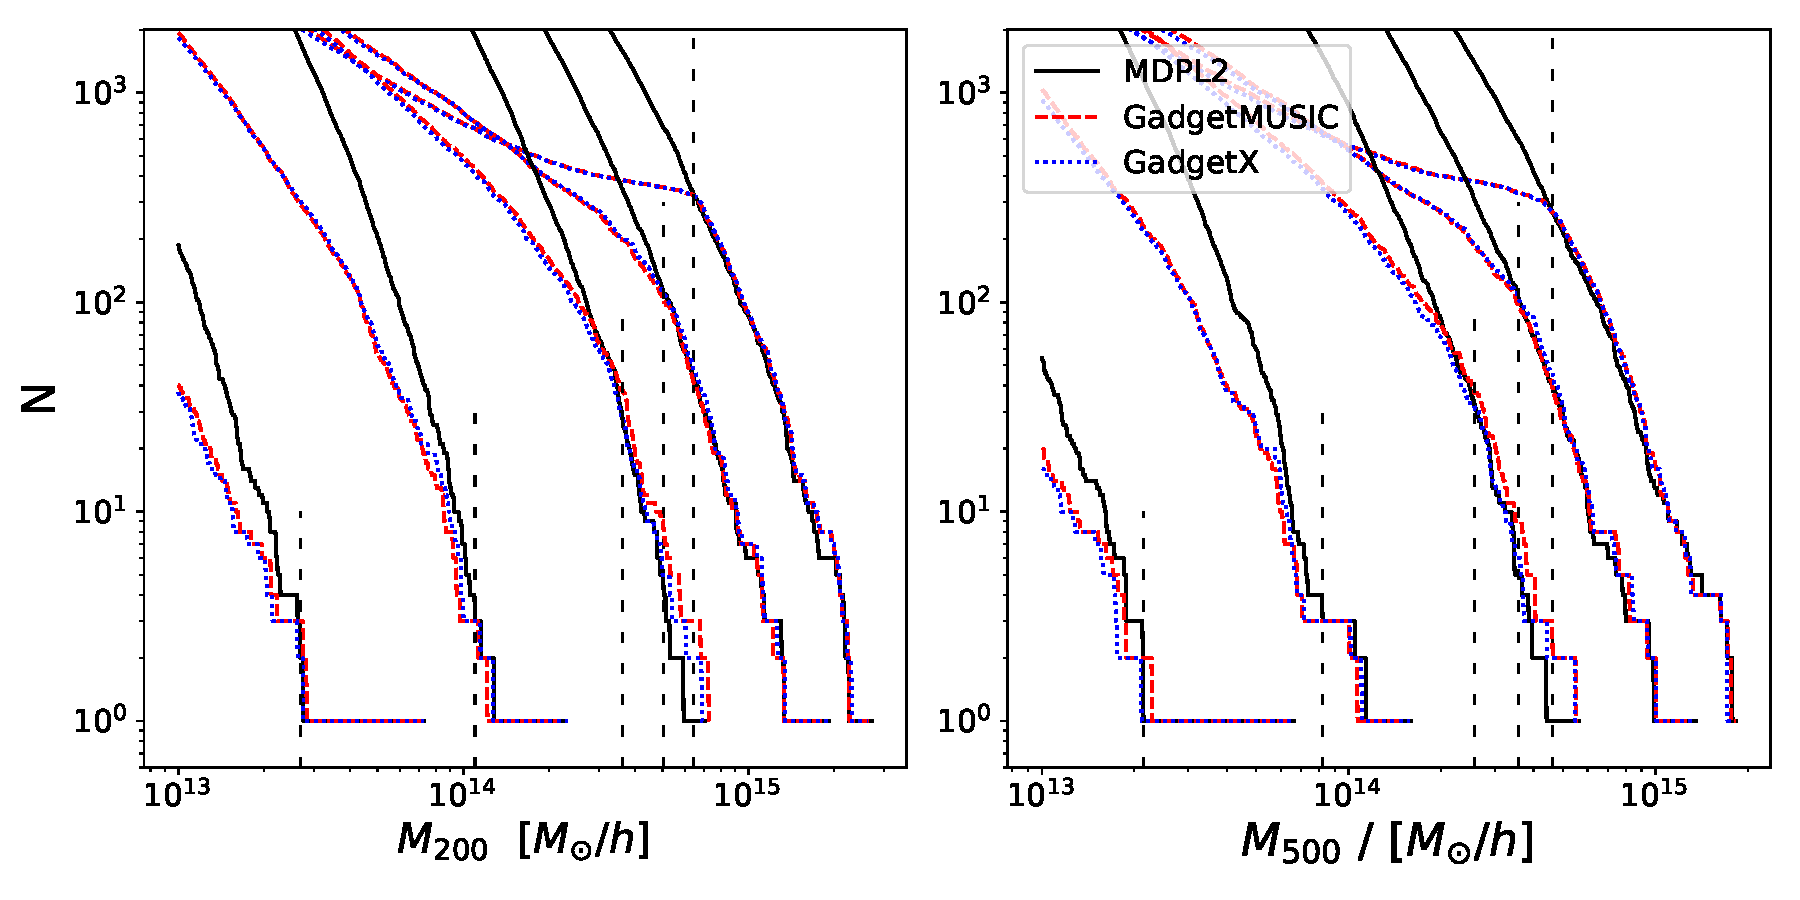
\includegraphics[width=0.9\textwidth]{HMF_full.pdf}
      \vspace{-0.5cm}
      \caption{Cumulative halo mass functions.}
    \end{figure}}
    \only<2>{
      \begin{table}
    	\centering
    	\caption{The \alert{mass-complete} sample of the Three Hundred cluster catalogues at different redshifts.}
    	\label{tab:masscomplete}
    	\begin{tabular}{lcccc} % four columns, alignment for each
    		\hline
    		redshift & $M_{200c}$  & $N_{200c}$ & $M_{500c}$  & $N_{500c}$ \\
            & [$10^{14} \hMsun$] & MUSIC/X & [$10^{14} \hMsun$] & MUSIC/X \\
            % &  & \gadgetmusic\ / \gadgetx\ & & \gadgetmusic\ / \gadgetx\ \\
    		\hline
    		  0.0		& \alert{6.42} & \alert{324 / 324} & \alert{4.6} & \alert{270 / 270}\\
    		  0.5		& 5.02 & 104 / 110 & 3.57 & 94 / 103\\
    		  1.0 	& 3.62 & 38 / 27   & 2.57 & 37 / 31 \\
          2.3 	& 1.10 & 3 / 3     & 0.82 & 3 / 3\\
          4.0 	& 0.27 & 3 / 2     & 0.21 & 2 / 1\\
    		\hline
    	\end{tabular}
    \end{table}
    }
\end{frame}

\section{The results}
\begin{frame}
  \begin{center}
    {\Huge The results} \\
    \bigskip
  \end{center}

  The results are mainly coming from
  \begin{itemize}
      \item     \hyperlink{intropaper}{\beamerbutton{\alert{the introduction paper}}} (Cui et al. 2018) is mainly about some general properites and scaling relations.
      \item \hyperlink{Wang}{\beamerbutton{the environment paper}} (Wang et al. 2018)  mainly talks about the differences between cluster and other environments.
      \item \hyperlink{Mostoghiu}{\beamerbutton{the density profile paper}} (Mostoghiu et al. 2018) studies the self-similarity of the density profiles in galaxy clusters.
      \item \hyperlink{Arthur}{\beamerbutton{The phase-space paper}} (Arthur et al. to be sumbitted) investigates the gas phase-space in and around galaxy clusters.
      \item \hyperlink{Li}{\beamerbutton{The physical density paper}} (Li et al. in final prep.) try to compare and understand the observable profiles in galaxy clusters.
  \end{itemize}
\end{frame}

\subsection{General Properties}\label{intropaper}
\begin{frame}
  \frametitle{General Properties: Baryon effects on halo mass}
  \only<1>{
  \begin{figure}
    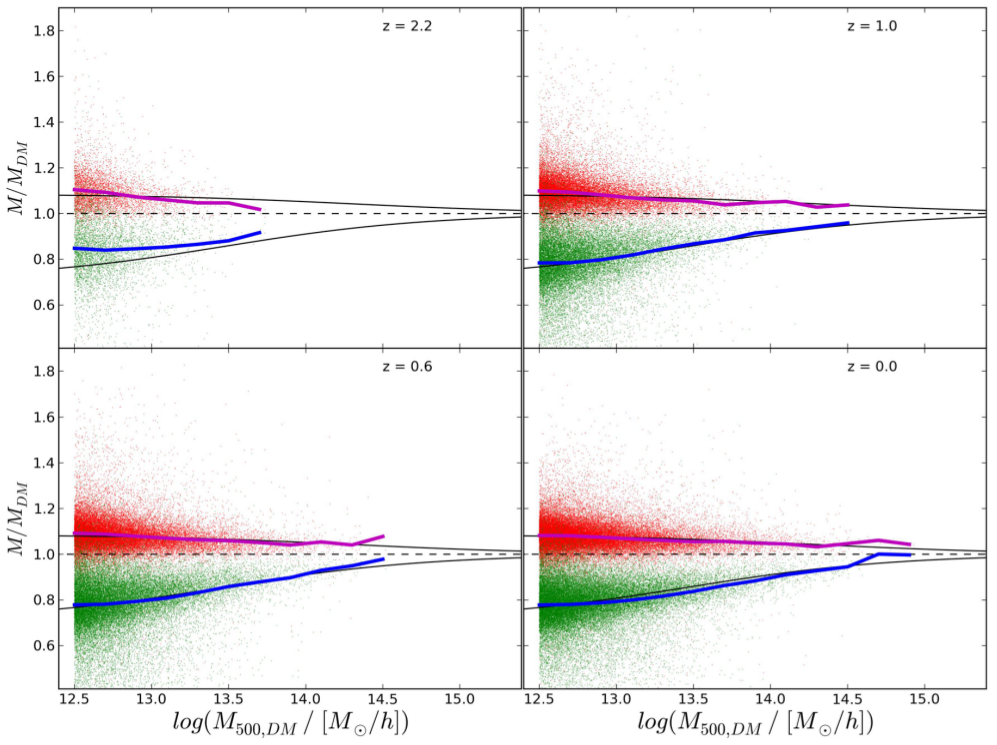
\includegraphics[width=0.7\textwidth]{Halo-mass-diff-cui2014}
    \vspace{-0.3cm}
    \caption{halo mass ($M_{500}$) difference respected to the DM run.\newline Ref: Cui et al. 2014}
  \end{figure}}
  \only<2>{
  \begin{figure}
    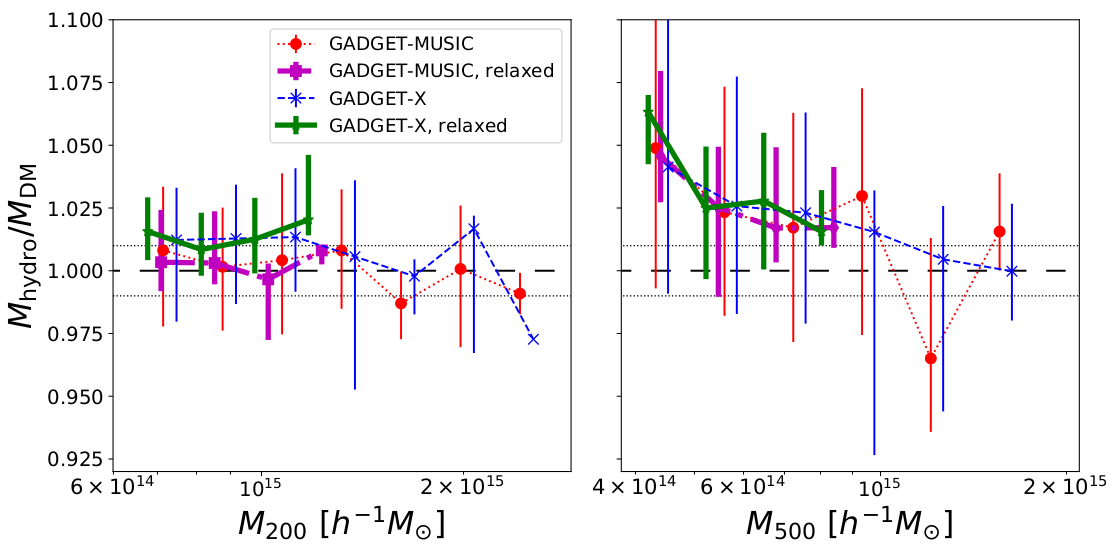
\includegraphics[width=\textwidth]{HMD-2}
    \vspace{-0.5cm}
    \caption{halo mass difference respected to the DM run.  }
  \end{figure}}
\end{frame}

\begin{frame}
  \frametitle{General Properties: the dynamical state}
  Classifying the cluster's dynamical state into relaxed and un-relaxed: the virial ratio $\eta = (2T-E_s)/|W|$ with $0.85 < \eta < 1.15$, center-of-mass offset $\Delta_r = |R_{cm} - R_{c}|/R_{200c}$ \textless 0.04 and subhalo mass fraction $f_s = \sum M_{sub}/M_{200c}$ \textless 0.1. Cui et al. 2017
  \only<1>{
    \begin{figure}
      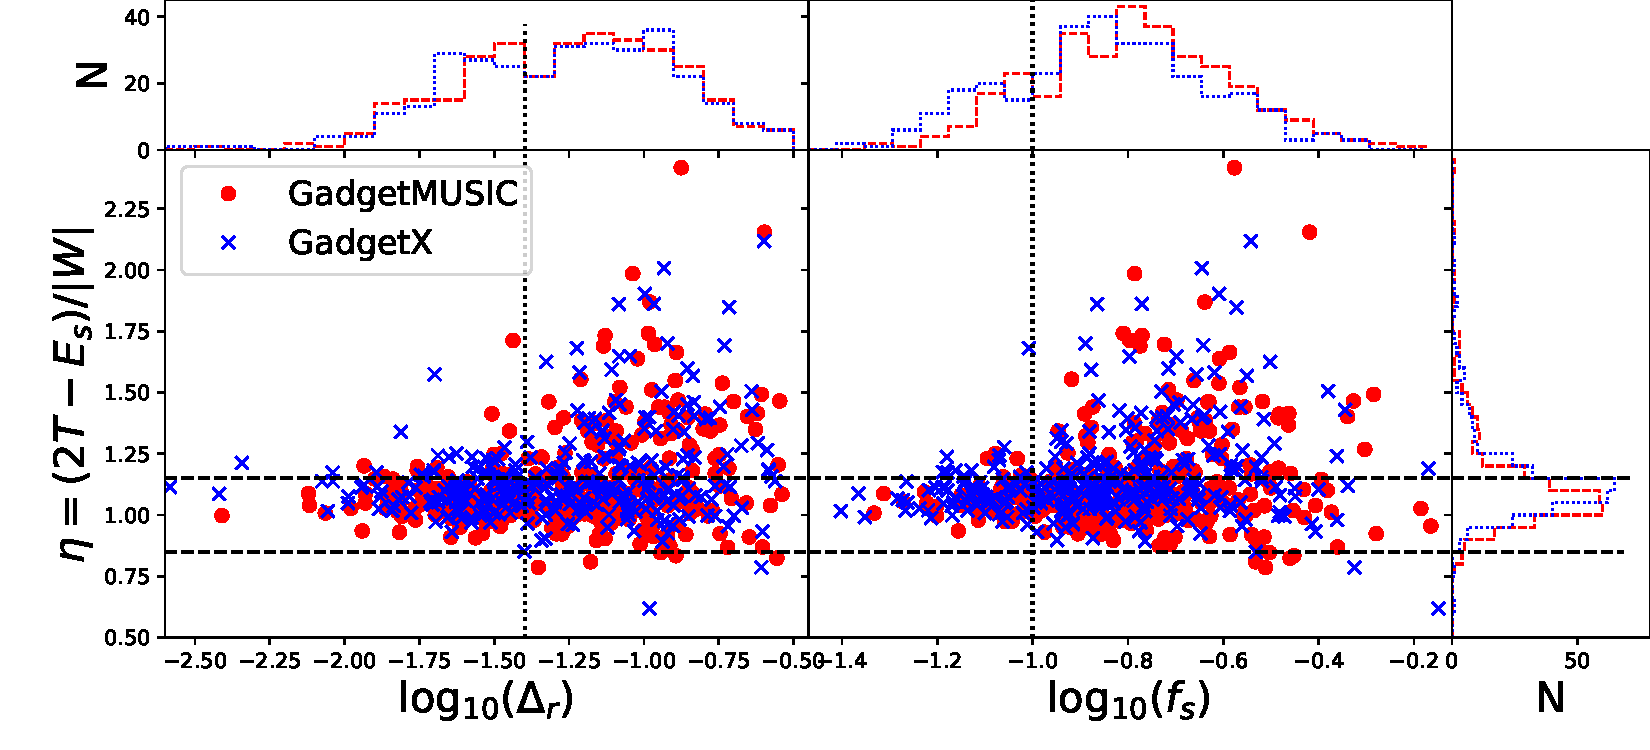
\includegraphics[width=0.9\textwidth]{ds-relations}
      \vspace{-0.4cm}
      \caption{The relations between the three parameters.}
    \end{figure}}
  \only<2>{
    \vspace{-0.8cm}
    \begin{columns}[t]
      \begin{column}{0.6\textwidth}
        \begin{table}
          \fontsize{7}{7}\selectfont
          \centering
          \caption{The fractions of relaxed clusters with different combinations of criteria.}
          \label{tab:relaxation}
          \begin{tabular}{lccc} % four columns, alignment for each
            \hline
            $M_{200c}$ & $\eta$, $\Delta_r$ \& $f_s$ & $\Delta_r$ \& $f_s$ & $f_s$ \\
            $10^{14} \hMsun$& MUSIC/X & MUSIC/X & MUSIC/X\\
            \hline
            $0.10 - 0.50$		& 0.44 / 0.36 & 0.56 / 0.48 & 0.70 / 0.65\\
            $0.50 - 1.00$		& 0.36 / 0.34 & 0.45 / 0.46 & 0.56 / 0.57\\
            $1.00 - 6.41$ 	& 0.27 / 0.29 & 0.30 / 0.35 & 0.43 / 0.48\\ \hdashline
            $>6.42$   	& \alert{0.15 / 0.17} & 0.16 / 0.21 & 0.17 / 0.23\\
            % \hline
          \end{tabular}
        \end{table}
      \end{column}
      \begin{column}{0.4\textwidth}
        \begin{table}
          \fontsize{7}{7}\selectfont
        	\centering
        	\caption{\scriptsize{The Cool Core cluster fraction (two methods: Rosetti et al. 2011 and central entropy) in the complete sample: $f_{CC} = \frac{N_{CC}}{N_{total}}$, the CC fraction in dynamically relaxed clusters $f_{CC/dr} = \frac{N_{CC, relaxed}}{N_{relaxed}}$ and the relaxation fraction in CC $f_{dr/CC} = \frac{N_{CC, relaxed}}{N_{CC}}$.}}
        	\label{tab:ccf}
        	\begin{tabular}{lccc} % four columns, alignment for each
        		\hline
        		Simulation & $f_{CC}$ & $f_{CC/dr}$ & $f_{dr/CC}$ \\
        		\hline
        		{\sc MUSIC}	& \alert{0.09} & 0.04 & 0.07\\
        		{\sc X} 		& \alert{0.26} & 0.33 & 0.21\\
        		% \hline
        	\end{tabular}
        \end{table}
      \end{column}
    \end{columns}
  }
\end{frame}

\begin{frame}{General properties: the concentration}
  \begin{figure}
    \includegraphics<1>[width=\linewidth]{C-M-relations}
    \vspace{-0.5cm}
    \caption{The concentration -- mass relation. Cui et al. 2018}
  \end{figure}
\end{frame}

\begin{frame}
  \frametitle{General Properties: the baryon fractions}
  \begin{figure}
    \includegraphics<1>[width=\linewidth]{Baryonic-fractions-hydro-full}
    % \vspace{-0.8cm}

    % \includegraphics<2>[width=\linewidth]{Baryonic-fractions-semi-full}
    \caption{The baryon fractions.  }
  \end{figure}
\end{frame}

\begin{frame}
  \frametitle{General Properties: the halo - central galaxy mass relation}
  \begin{figure}
    \includegraphics<1>[width=0.7\linewidth]{HS-relation-full}
    \vspace{-0.5cm}
    \caption{The halo mass - central galaxy mass relation.}
  \end{figure}
\end{frame}

\subsubsection{Scaling relations}
\begin{frame}
  \frametitle{Optical relations}
  The complete sample is used here.
  \begin{figure}
    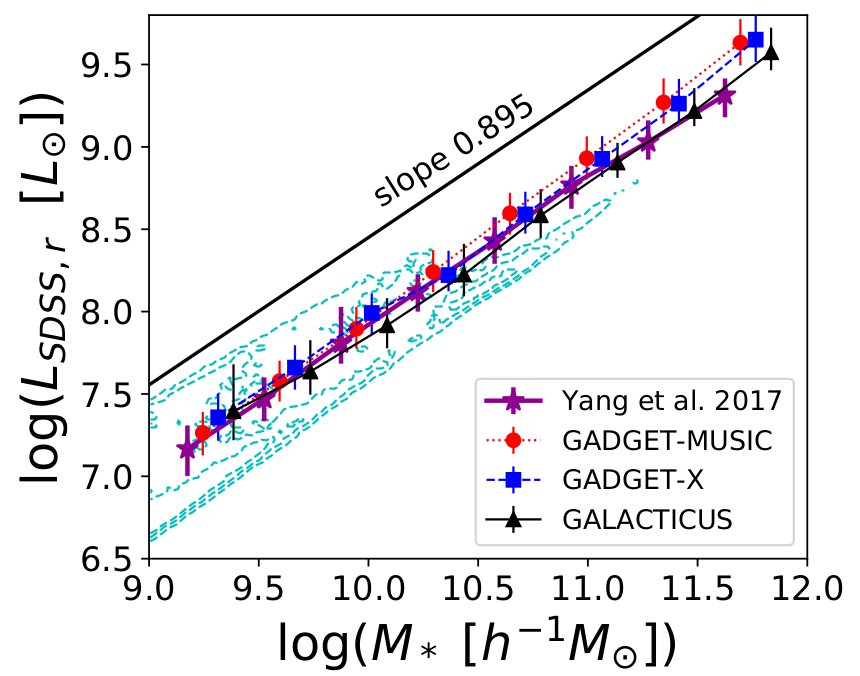
\includegraphics[width=0.33\linewidth]{Optical-relation1}
    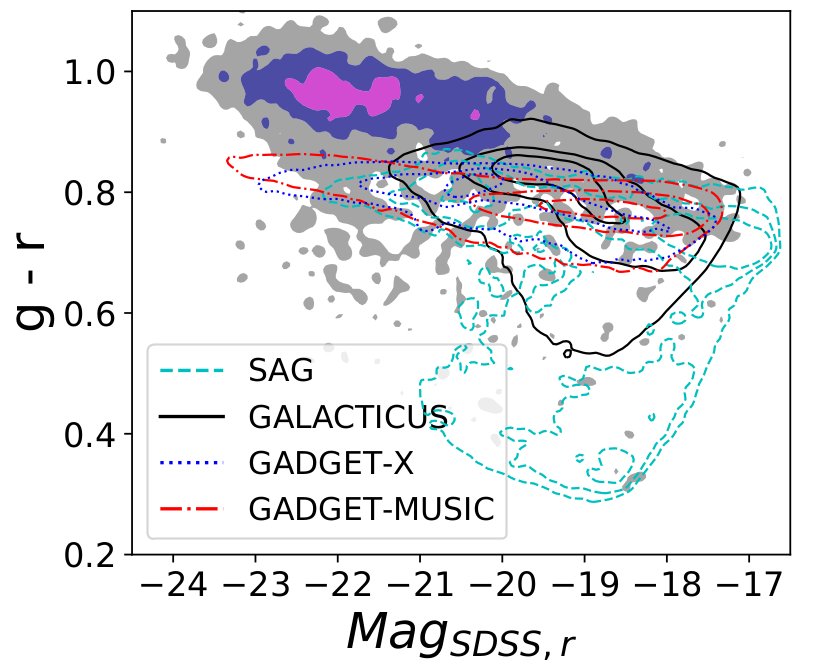
\includegraphics[width=0.32\linewidth]{Optical-relation2}
    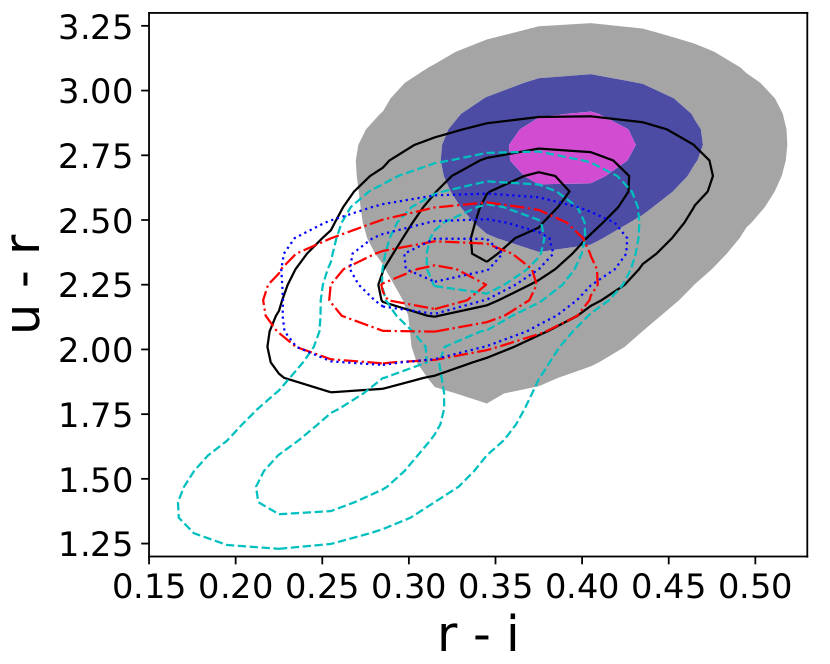
\includegraphics[width=0.32\linewidth]{Optical-relation3}
    \vspace{-0.3cm}
    \caption{The optical relations.  }
  \end{figure}
\end{frame}
\begin{frame}
  \frametitle{Optical relations: the satellite stellar mass function}
  The complete sample is used here.
  \begin{figure}
    \includegraphics<1>[width=0.7\linewidth]{Ssmf}
    \vspace{-0.6cm}
    \caption{The satellite stellar mass function.  }
  \end{figure}
\end{frame}

\begin{frame}
  \frametitle{Gas scaling relations}
  \begin{figure}
    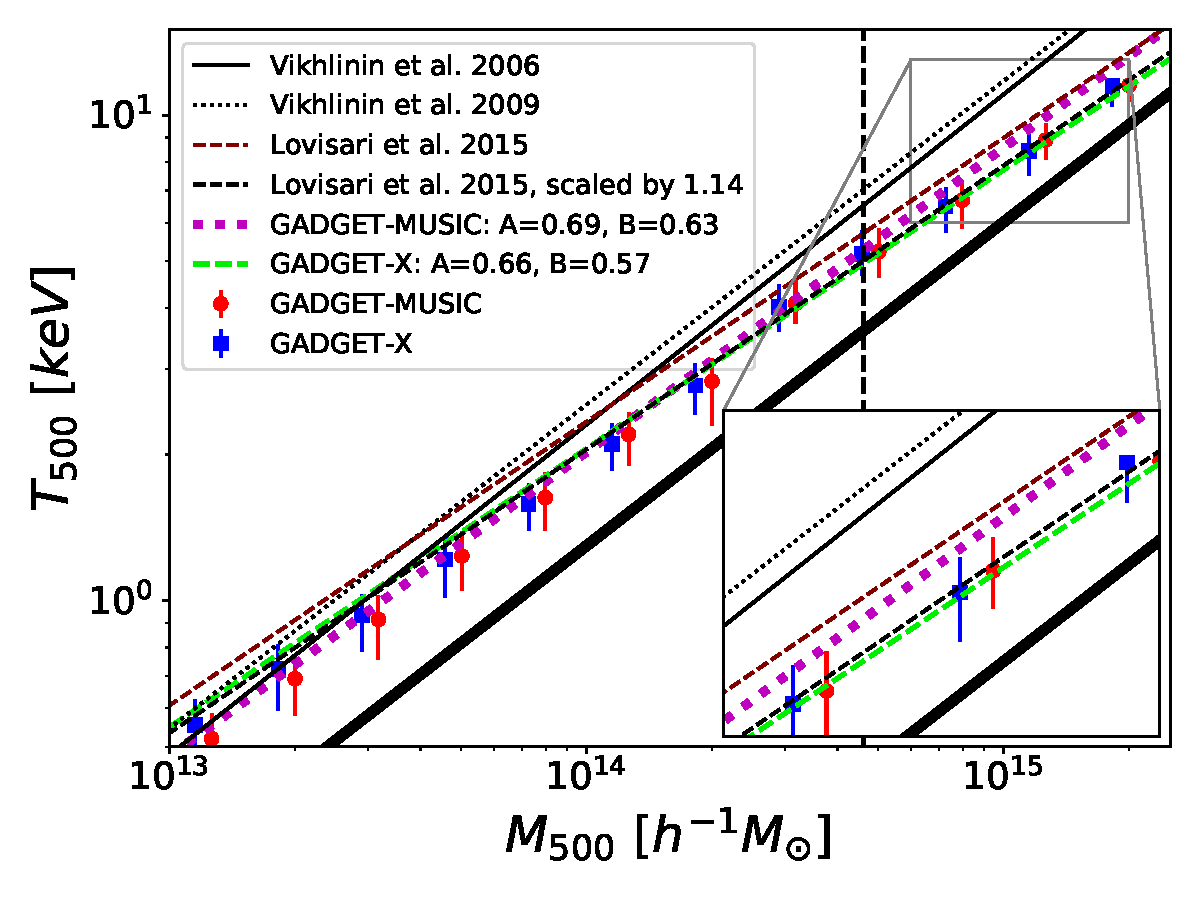
\includegraphics[width=0.48\linewidth]{T-M-relations}
    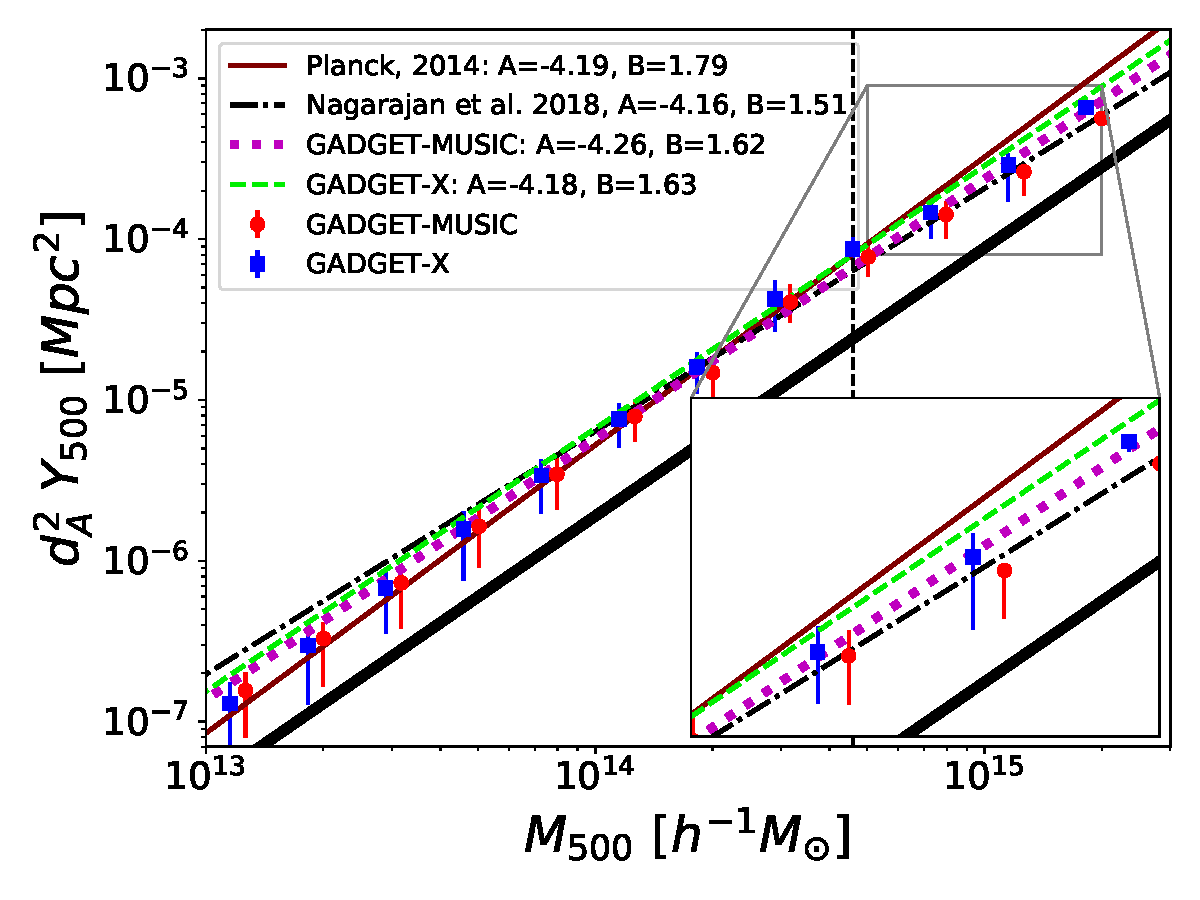
\includegraphics[width=0.48\linewidth]{YM_relation-full.pdf}
    \vspace{-0.4cm}
    \caption{The gas scaling relations.}
  \end{figure}

\begin{center}
  Fitting function -- $Y_{500} = 10^A (\frac{M_{500}}{6\times10^{14} M_{\odot}})^B$
\end{center}
\end{frame}

\begin{frame}{Conclusion 1}
  {
  \begin{itemize}
    \item The baryons have a negligible impact on the halo mass for both $M_{200}$ and $M_{500}$.
    \item $\sim 20 \%$ of the complete sample is relaxed clusters, 26\% (9\%) of the sample is CC for GadgetX (MUSIC).
    \item Compare with observations (Agreement): The baryon fractions for cluster mass range, optical relations and gas scaling relations are generally in agreement with the observations.
    \item Compare with observations (Disagreement):  stellar-halo mass relation (A problem of ICL), galaxy color in clusters seems a little blue.
  \end{itemize}}
  \begin{center}
    \hyperlink{lastpage}{\beamerbutton{jump to the last slide}}    
  \end{center}
\end{frame}

\begin{frame}
  \begin{center}
    {\Huge The results} \\
    \bigskip
  \end{center}
  
  \begin{itemize}
      \item     \hyperlink{intropaper}{\beamerbutton{the introduction paper}} (Cui et al. 2018) is mainly about some general properites and scaling relations.
      \item \hyperlink{Wang}{\beamerbutton{\alert{the environment paper}}} (Wang et al. 2018)  mainly talks about the differences between cluster and other environments.
      \item \hyperlink{Mostoghiu}{\beamerbutton{the density profile paper}} (Mostoghiu et al. 2018) studies the self-similarity of the density profiles in galaxy clusters.
      \item \hyperlink{Arthur}{\beamerbutton{The phase-space paper}} (Arthur et al. to be sumbitted) investigates the gas phase-space in and around galaxy clusters.
      \item \hyperlink{Li}{\beamerbutton{The physical density paper}} (Li et al. in final prep.) try to compare and understand the observable profiles in galaxy clusters.
  \end{itemize}
\end{frame}

\subsection{The environment effects}\label{Wang}
\begin{frame}{The environment effects: the aims}
    We seek to understand the relationship between galaxy properties and their host environment (overdensity measuaged within $1\Mpc$ -- $\sigma_1$) as well as three large scale different environments: cluster, vicinity and void. 
    
    Only GadgetX results are used.
\end{frame}
\begin{frame}{The environment effects: Wang et al. 2018}
  \only<1>{
  \begin{center}
        \begin{tikzpicture}
            \node[anchor=south west,inner sep=0] at (0,0) {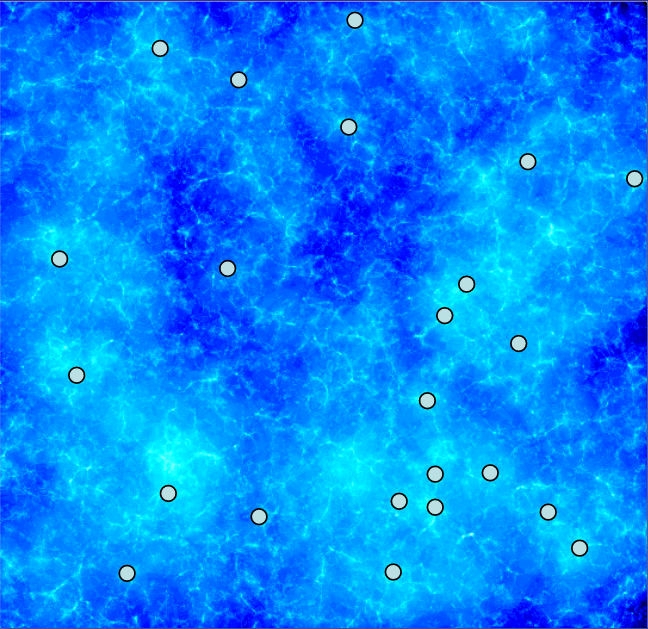
\includegraphics[width=0.6\linewidth]{MDPL2}};
            \draw[red,ultra thick] (4,4.7) circle (0.5cm);
            \draw[magenta,thick] (1.89,1.53) circle (0.2cm);
        \end{tikzpicture}
    \end{center}
    \begin{textblock}{0.25}(0.02,0.2)
      {\scriptsize Three environments: cluster ($<2*R_{200}$); vicinity ($2*R_{200} - 10\Mpc$ and Void ($<38 \Mpc$).}
    \end{textblock}
  }
  \only<2>{
  \begin{figure}
    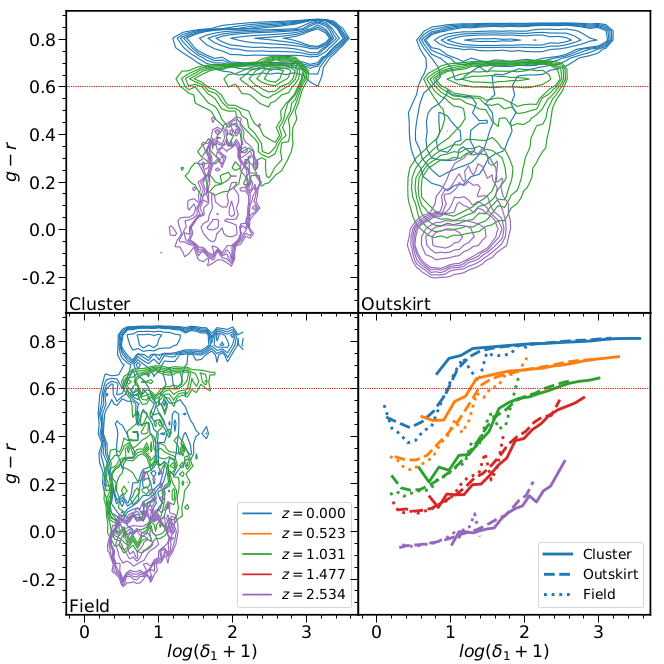
\includegraphics[width=0.6\linewidth]{Yang-color}
    \vspace{-0.4cm}
    \caption{color--environment relation. credit: Wang et al. 2018}
  \end{figure}
  }
  \only<3>{
    \begin{figure}
    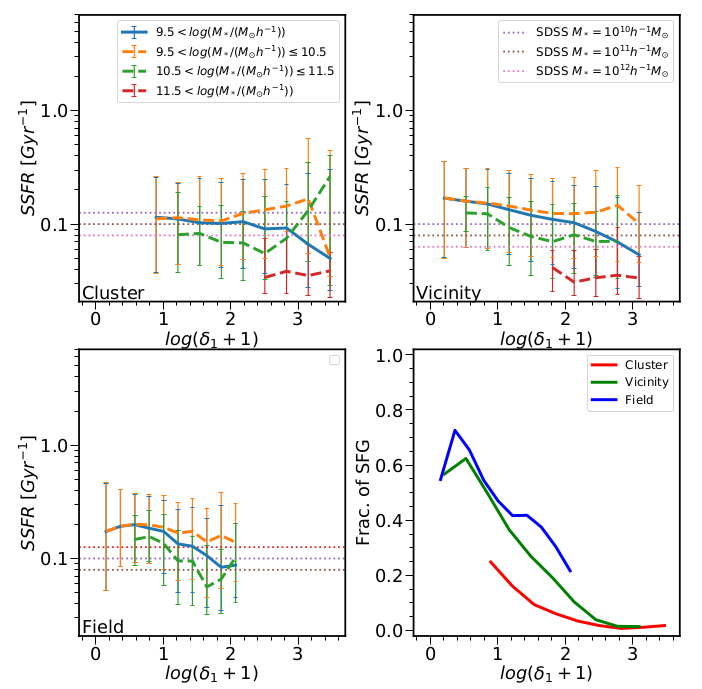
\includegraphics[width=0.6\linewidth]{Yang-sSFR}
    \vspace{-0.4cm}
    \caption{sSFR -- environment relation. credit: Wang et al. 2018}
  \end{figure}}
  \only<4>{
  \begin{figure}
    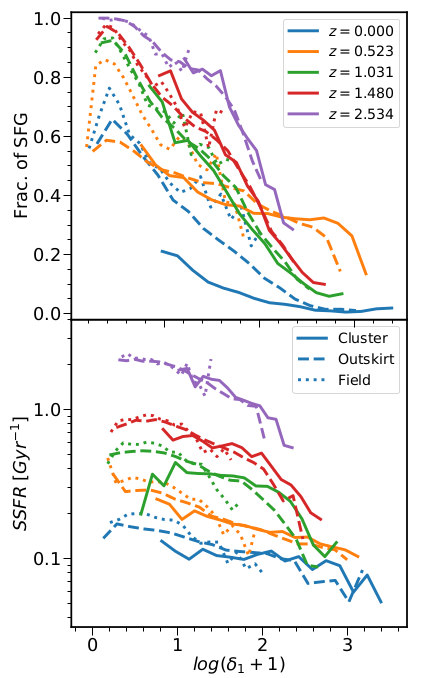
\includegraphics[width=0.4\linewidth]{Yang-SFR}
    \vspace{-0.6cm}
    \caption{SFR -- environment relation. credit: Wang et al. 2018}
  \end{figure}
  }
\end{frame}
\begin{frame}{Conclusion 2}
  \begin{itemize}
    \item As expected, galaxies in denser environments tend to be redder and are more likely to be quenched.
    \item Although the sSFR decreases with $\sigma_1$, this is mainly because that galaxies with higher stellar mass reside in environment with higher overdensity. 
    \item At fixed over-density a galaxy's colour is also independent of whether it lives within a cluster or within the field, but the relative fractions of the two samples varies dramatically with over-density and this drives an apparent evolution.
  \end{itemize}
    \begin{center}
    \hyperlink{lastpage}{\beamerbutton{jump to the last slide}}    
  \end{center}
\end{frame}

\begin{frame}
  \begin{center}
    {\Huge The results} \\
    \bigskip
  \end{center}
  
  \begin{itemize}
      \item     \hyperlink{intropaper}{\beamerbutton{the introduction paper}} (Cui et al. 2018) is mainly about some general properites and scaling relations.
      \item \hyperlink{Wang}{\beamerbutton{the environment paper}} (Wang et al. 2018)  mainly talks about the differences between cluster and other environments.
      \item \hyperlink{Mostoghiu}{\beamerbutton{\alert{the density profile paper}}} (Mostoghiu et al. 2018) studies the self-similarity of the density profiles in galaxy clusters.
      \item \hyperlink{Arthur}{\beamerbutton{The phase-space paper}} (Arthur et al. to be submitted) investigates the gas phase-space in and around galaxy clusters.
      \item \hyperlink{Li}{\beamerbutton{The physical density paper}} (Li et al. in final prep.) try to compare and understand the observable profiles in galaxy clusters.
  \end{itemize}
\end{frame}

\subsection{The density profiles}\label{Mostoghiu}
\begin{frame}{The cluster density profiles: Mostoghiu et al. 2018.}
  \begin{columns}[t]
    \begin{column}{0.3\textwidth}
      \begin{figure}
        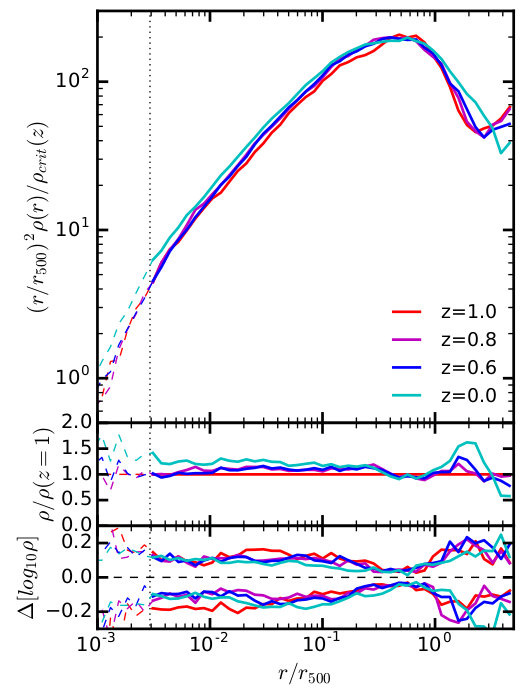
\includegraphics[width=\linewidth]{LeBrun18}
        \caption{Density profiles. Le Brun et al. 2018}
      \end{figure}
    \end{column}
    \begin{column}{0.7\textwidth}
      \only<1>{
      \begin{figure}
        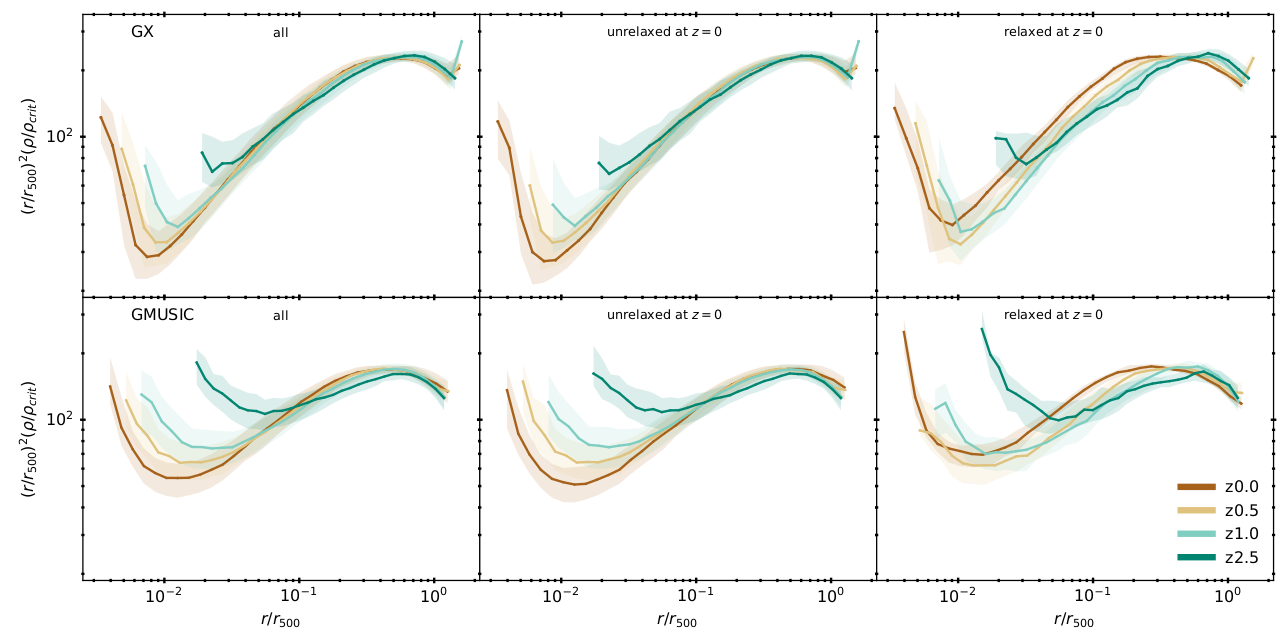
\includegraphics[width=\linewidth]{Robert-density}
        \caption{Density profiles from the mass-complete sample. credit: Robert Mostoghiu}
      \end{figure}}
      \only<2>{
      \begin{figure}
        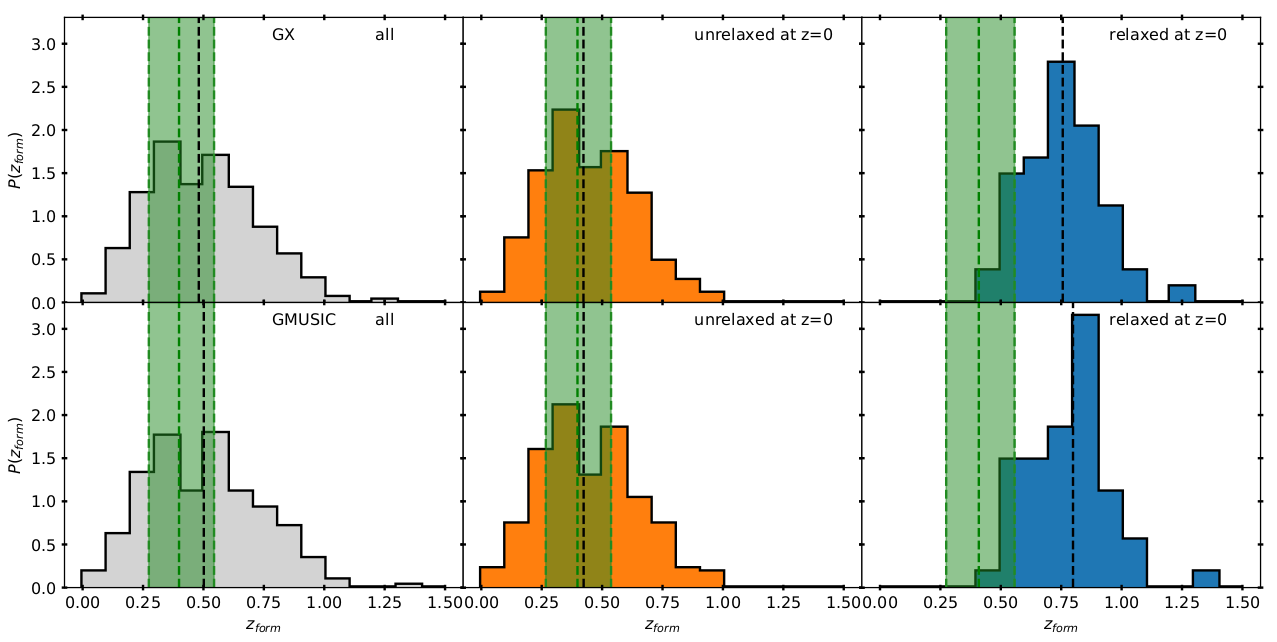
\includegraphics[width=\linewidth]{Robert-formationtime}
        \caption{Formation time. credit: Robert Mostoghiu}
      \end{figure}}
    \end{column}
  \end{columns}
\end{frame}
\begin{frame}{Conclusion 3}
 
  \begin{itemize}
    \item Relaxed clusters show a weak redshift evolution of the density profile, which is due to their earlier formation time.
  \end{itemize}
    \begin{center}
    \hyperlink{lastpage}{\beamerbutton{jump to the last slide}}    
  \end{center}
\end{frame}

\begin{frame}
  \begin{center}
    {\Huge The results} \\
    \bigskip
  \end{center}

  \begin{itemize}
      \item     \hyperlink{intropaper}{\beamerbutton{the introduction paper}} (Cui et al. 2018) is mainly about some general properites and scaling relations.
      \item \hyperlink{Wang}{\beamerbutton{the environment paper}} (Wang et al. 2018)  mainly talks about the differences between cluster and other environments.
      \item \hyperlink{Mostoghiu}{\beamerbutton{the density profile paper}} (Mostoghiu et al. 2018) studies the self-similarity of the density profiles in galaxy clusters.
      \item \hyperlink{Arthur}{\beamerbutton{\alert{The phase-space paper}}} (Arthur et al. to be sumbitted) investigates the gas phase-space in and around galaxy clusters.
      \item \hyperlink{Li}{\beamerbutton{The physical density paper}} (Li et al. in final prep.) try to compare and understand the observable profiles in galaxy clusters.
  \end{itemize}
\end{frame}

\subsection{The gas phase-space distribution}\label{Arthur}
\begin{frame}{The gas phase-sapce distribution}

\end{frame}
\begin{frame}{Conclusion 4}
  \begin{itemize}
    \item The baryons have a negligible impact on the halo mass for both $M_{200}$ and $M_{500}$.
  \end{itemize}
    \begin{center}
    \hyperlink{lastpage}{\beamerbutton{jump to the last slide}}    
  \end{center}
\end{frame}

\begin{frame}
  \begin{center}
    {\Huge The results} \\
    \bigskip
  \end{center}

  \begin{itemize}
      \item     \hyperlink{intropaper}{\beamerbutton{the introduction paper}} (Cui et al. 2018) is mainly about some general properites and scaling relations.
      \item \hyperlink{Wang}{\beamerbutton{the environment paper}} (Wang et al. 2018)  mainly talks about the differences between cluster and other environments.
      \item \hyperlink{Mostoghiu}{\beamerbutton{the density profile paper}} (Mostoghiu et al. 2018) studies the self-similarity of the density profiles in galaxy clusters.
      \item \hyperlink{Arthur}{\beamerbutton{The phase-space paper}} (Arthur et al. to be sumbitted) investigates the gas phase-space in and around galaxy clusters.
      \item \hyperlink{Li}{\beamerbutton{\alert{The physical density paper}}} (Li et al. in final prep.) try to compare and understand the observable profiles in galaxy clusters.
  \end{itemize}
\end{frame}

\subsection{The observable profiles}\label{Li}
\begin{frame}{The observable profiles}

\end{frame}
\begin{frame}{Conclusion 5}
  {
  \begin{itemize}
    \item The baryons have a negligible impact on the halo mass for both $M_{200}$ and $M_{500}$.
  \end{itemize}}
\end{frame}

\section{future prospects}\label{lastpage}
\begin{frame}
  \frametitle{Future works}
  \begin{itemize}
    \item<1|only@1>[]{
    \begin{figure}
      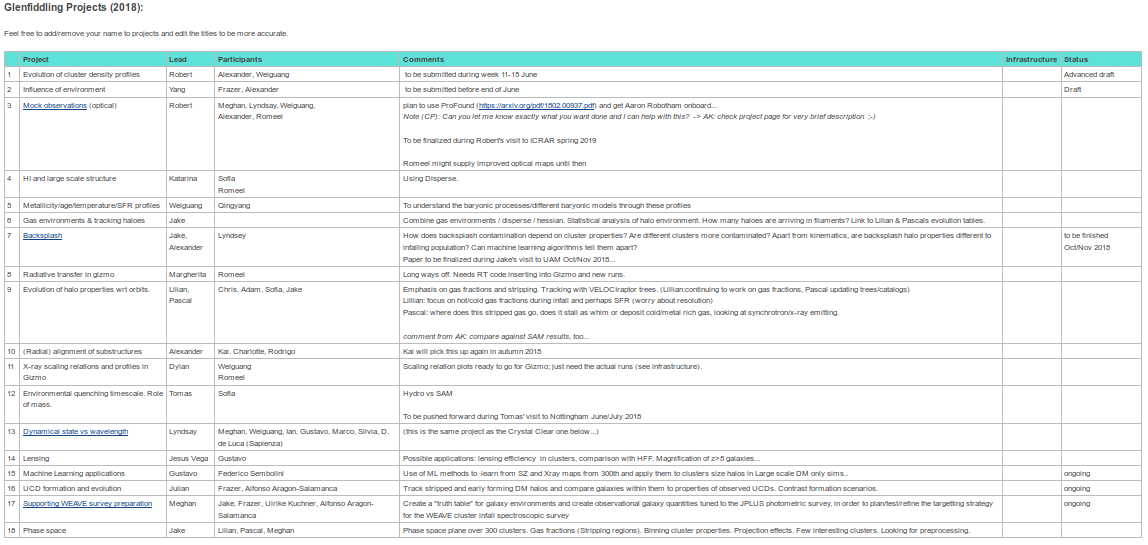
\includegraphics[width=\linewidth]{Tasks18}
      \caption{Tasks from GlenFindding workshop.}
    \end{figure}}
    \item<2|only@2>[]{
      \begin{figure}
        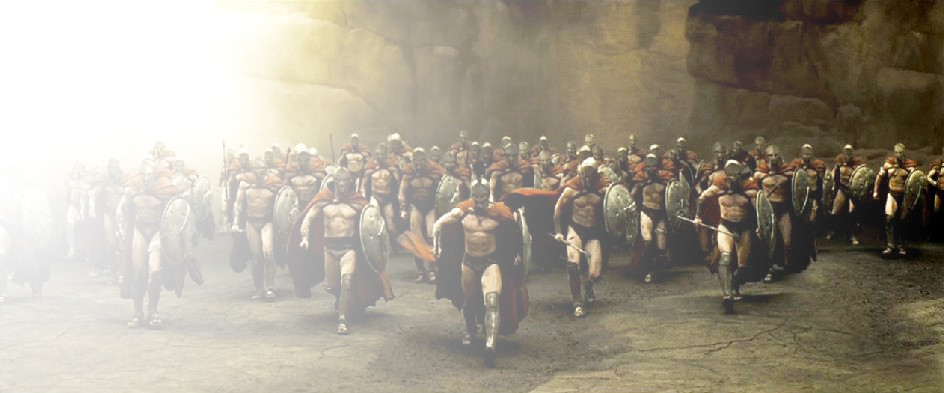
\includegraphics[width=\linewidth]{The300}
        \caption{Be one of us!}
      \end{figure}
      Contact me \alert{cuiweiguang@gmail.com}, Alexander \alert{alexander.knebe@uam.es} or Gustavo \alert{gustavo.yepes@uam.es}}
  \end{itemize}

\end{frame}
\end{document}
